% APS Open Science submission candidate for author review, 2026-10-28
\documentclass[%
  aps,physrev,onecolumn,10pt,amsmath,amssymb,superscriptaddress,longbibliography,floatfix
]{revtex4-2}

\usepackage{graphicx}
% REVTeX 4.2f requires the legacy array implementation on TeX Live 2025.
\usepackage{array}[=2016-10-06]
\usepackage{dcolumn}
\usepackage{bm}
\usepackage{physics}
\usepackage{hyperref}
\hypersetup{hidelinks,pdfauthor={Vinayak M. Kulkarni},pdftitle={Emergent PT Symmetry and Exceptional Points in a Driven Dirac Impurity}}
\pdfstringdefDisableCommands{\def\PT{PT}\def\({}\def\){}\def\tb{beta}\def\gb{beta0}}
\usepackage{xcolor}
\usepackage{booktabs}
\usepackage{enumitem}
\usepackage{placeins}
\usepackage{xr-hyper}

\newcommand{\PT}{\mathcal{PT}}
\newcommand{\Hss}{H_{\rm ss}}
\newcommand{\Htilde}{\tilde{H}}
\newcommand{\teps}{\tilde{\epsilon}_{\xi}}
\newcommand{\keff}{\kappa_{\rm imp}}
\newcommand{\Gless}{G^{<}}
\newcommand{\Gret}{G^{R}}
\newcommand{\Gadv}{G^{A}}
\newcommand{\tb}{\tilde{\beta}}          % gauge-invariant SBMF scale
\newcommand{\gb}{\beta_0}               % signed frozen drive-control amplitude
\newcommand{\Gpt}{\Gamma_{\mathrm{PT}}}   % projected gain/loss channel
\newcommand{\dSig}{\delta_{\Sigma}}          % real one-body self-energy shift
\newcommand{\Deff}{\Delta_{\rm eff}}     % projected coherent splitting/flip
\newcommand{\Dzero}{\Delta_0}              % static coherent splitting in generic projection
\newcommand{\Dcoh}{\Delta_{\rm coh}}          % Kramers--Kronig coherent detuning
\newcommand{\Veff}{V_{\rm eff}}           % projected impurity-bath hybridization
\newcommand{\cV}{c_V}

\externaldocument[M-][nocite]{main}
\begin{document}
\title{Supplemental Material for ``Emergent \texorpdfstring{$\PT$}{PT} Symmetry and Exceptional Points in a Driven Dirac Impurity''}
\author{Vinayak M.~Kulkarni}
\thanks{JNCASR is the author's doctoral affiliation; this work was carried out independently}
\affiliation{Theoretical Sciences Unit,
  Jawaharlal Nehru Centre for Advanced Scientific Research,
  Jakkur, Bangalore 560064, India}
\date{October 28, 2026}
\maketitle
\setcounter{figure}{0}
\renewcommand{\thefigure}{S\arabic{figure}}

This Supplemental Material gives the derivations, certificates, and validation checks that support the main article.
Throughout, $\PT$ denotes parity--time symmetry.

\section*{Notation and parameter conventions}
\begin{description}[leftmargin=1.6cm,style=nextline]
\item[$t_{\rm av},\tau,T_{\rm b}$]
Wigner center time $(t+t')/2$, relative time $t-t'$, and reservoir temperature.
\item[$\eta,\zeta_\sigma$]
Chiral bath index $\eta=\pm$ and spin sign $\zeta_\uparrow=+1$, $\zeta_\downarrow=-1$.
\item[$\lambda,j_\alpha,\chi_K$]
SOC strength, eigenvalues of the bath-density-normalized Schrieffer--Wolff
matrix $\rho_b^{1/2}J^{\rm SW}\rho_b^{1/2}$, and the one-loop coefficient
defined by $dj/d\ell=\chi_Kj^2$.  For an antiferromagnetic Hermitian
reference, $j_{\rm scr}$ denotes the largest positive eigenvalue.
\item[$\alpha_{\rm b},k_{\rm max},D_{\rm uv}$]
Quadratic bath-dispersion coefficient, radial momentum cutoff, and ultraviolet
energy cutoff.  The normalized $k=0$ core figures contain neither cutoff;
$k_{\rm max}=\pi/4$ is used in the causal gate and
$D_{\rm uv}=\pi/4$ only in the sharp-cutoff reachability audit.
\item[$\epsilon_\xi,\epsilon_d,\tilde\epsilon_\xi$]
Bare impurity gate in the benchmark notation, bare gate in the full-bath
calculation, and renormalized level of the scalar slave-boson benchmark.
The latter includes the real constraint and projected one-body shifts.
\item[$W_k,W,\Lambda_\eta^{\rm PV}$]
Static bare impurity--bath hybridization and principal-value bath shift.
The drive does not set $W_k$; at the saddle the vertex is $rW_k$.
\item[$\beta_0,\tilde\beta$]
Signed frozen drive-control amplitude and nonnegative slave-boson mean-field
(SBMF) projection $\tilde\beta=|\beta_0||b_c|$.  On the two paths described
below the table, $G=|\beta_0|$ or $G=0.20\beta_0$, so $\beta_0$ is not itself
a decay rate.
\item[$z,z_W,s$]
Complex frequency, Wilson discretization shift, and frozen-core half-splitting
($E_+-E_-=2s$).  The physical retarded boundary is
$z=\mu+\omega+i0^+$ when $\omega$ is measured from $\mu$;
$\zeta_\sigma$ denotes the spin sign.
\item[$\mathsf{s}_a,\delta_a$]
Eigenvalues $\mathsf{s}_a=e^{2i\delta_a}$ and eigenphases of the complete
unitary scattering matrix.  They are distinct from the EP pole splitting $s$ and from the fixed chiral labels $\eta=\pm$.
\item[$D,G,\Gamma_{\rm PT},\bar\Gamma$]
Constant-core coherent splitting, constant-core relative channel, projected
relative decay imbalance, and common bath width.  The symbols
$\tilde\Gamma_\eta$ and $\Gamma_\sigma^{\rm net}$ denote, respectively, the
chiral frozen-kernel width and the physical net channel width.
\item[$\omega,\Omega,\omega_0$]
Fourier frequency, drive frequency, and a selected spectral pole or resonance frequency; none of these denotes temperature.
\item[$\mathcal E_n,E_{\rm EP},\Lambda(\omega)$]
Non-Hermitian eigenvalues, EP eigenvalue, and real bath self-energy.
\item[$\mathcal P,\mathfrak a,\mathfrak b$]
Full-kernel Schur polynomial and the two local contact denominators; these are distinct from the bath coefficient $\alpha_{\rm b}$.
\item[$\mathcal F_{\rm dist},\mathcal F_{\rm MF}$]
Distribution matrix and mean-field free-energy functional.
\item[$R,\Lambda_f,D_d$]
Finite-$U$ Kotliar--Ruckenstein renormalization matrix and constraint field
(App.~\ref{app:KR}), and impurity double occupancy
$\langle n_{d\uparrow}n_{d\downarrow}\rangle$.  The constraint field is distinct
from the Wilson parameter $\Lambda$ and the real bath self-energy $\Lambda(\omega)$.
\end{description}

For clarity, the same constant two-component matrix is written in three
conventions:
\begin{center}
\begin{tabular}{@{}lll@{}}
\toprule
representation & constant matrix & identification \\
\midrule
spin basis & $D\sigma_x+iG\sigma_z$ & $D=\Deff$, $G=\Gpt$ \\
fixed chiral basis & $D\sigma_z+iG\sigma_x$ & Hadamard rotation \\
companion algebra & $\gamma\sigma_x+i\beta\sigma_z$ & $\gamma=D$, $\beta=G$ \\
\bottomrule
\end{tabular}
\end{center}
The frozen drive coordinate is instead $\beta_0$; it must not be identified
with the matrix coefficient $G$ or with the companion symbol $\beta$.
The normalized geometry plots use $D=0.50$ and $G=|\beta_0|$, whereas the
small-width causal/flow audit uses $D=0.075+0.050\beta_0$ and
$G=0.20\beta_0$, giving $D=0.10$ at the core point.  The geometry path has crossings at $\beta_0=\pm0.50$;
the small-width audit uses only $0.35\leq\beta_0\leq0.55$ and crosses
at $\beta_0=0.50$.  These are different parameter paths, with neither
identical coherent coefficients nor identical physical decay rates.

\appendix
% ============================================================

\section{Impurity-block EP condition and condition-number scaling}
\label{app:harmonic}
\label{app:EP_scaling}

This appendix records the impurity-block algebra used in the main text.
The Hadamard rotation itself is shown in
Eq.~(\ref{M-eq:Htilde}); here we keep only
the EP and condition-number scaling that underlies the diagnostic
interpretation.

The frozen impurity block is
$h_d=\bigl[\begin{smallmatrix}\teps+D&iG\\iG&\teps-D
\end{smallmatrix}\bigr]$, with eigenvalues $E_\pm=\teps\pm s$
and splitting $s=\sqrt{D^2-G^2}$.  The regimes are
$\PT$-unbroken ($D>G$), exceptional ($D=G$), and
$\PT$-broken ($G>D$) for positive parameters.  Right eigenvectors may be
chosen as $|r_\pm\rangle=[G,\,i(D\mp s)]^T$, so $\det R=2iG s, \qquad R=(|r_+\rangle,|r_-\rangle)$.
Thus, near the bare EP,
\begin{equation}
\keff=\|R\|\|R^{-1}\|\sim\frac{C}{|s|},
\label{eq:kappa_scaling}
\end{equation}
with a nonsingular constant $C$.  The standard local \(U\) does not cut off
this algebraic divergence on the equal-velocity, scalar-hybridization
linearized submanifold because it preserves the complexified pseudospin
symmetry.  At fixed real frequency with a strictly positive decay margin, the
complete retarded resolvent stays finite despite the singular eigenbasis;
the analytically continued Green function still has its resonance poles.  Curvature, unequal velocities, frequency dependence, or
component-dependent vertices can lift the exact symmetry and must be
analyzed separately.

\begin{figure}[htbp]
\centering
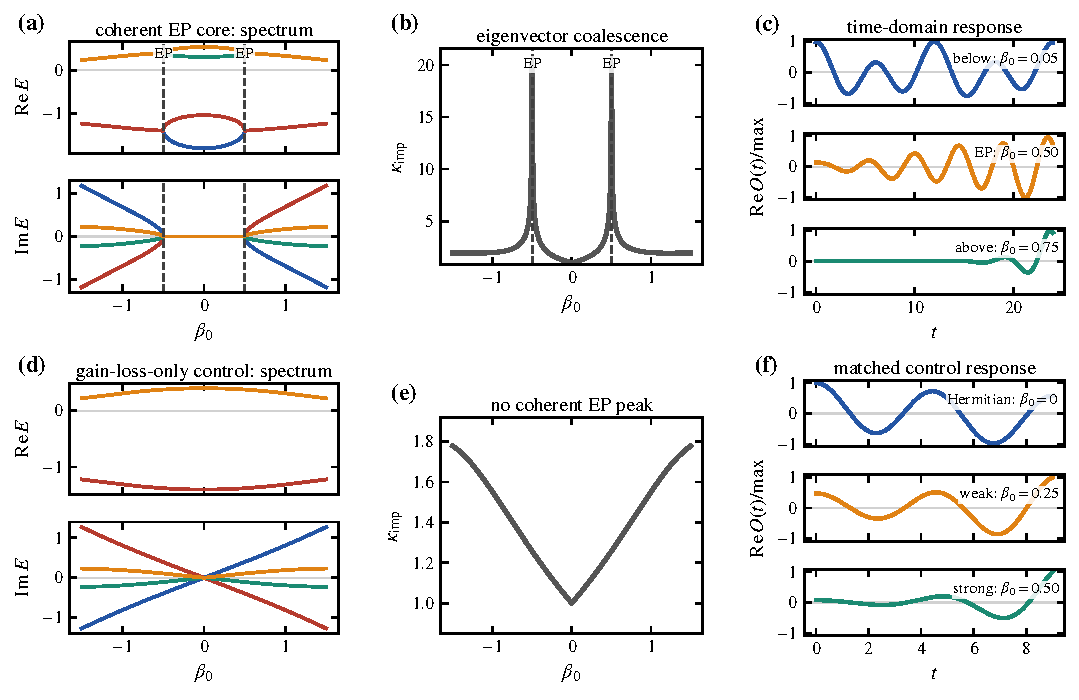
\includegraphics[width=0.90\textwidth]{Fig4_frozen_kernel.pdf}
\caption{%
\textbf{Frozen $4\times4$ compensated-core EP and matched control.}
All panels use the rotated kernel of Eq.~(\ref{M-eq:Htilde}) at $k=0$ with
$r=1$, $\teps=-1$, fixed scalar hybridization $W=0.75$, and
$G=\Gamma_{\rm PT}=|\beta_0|$.  The level $\teps=-1$ is an assigned benchmark coefficient; the historical
label $\epsilon_\xi=-U/2$ at $U=2$ is not an interaction calculation.
No microscopic bath DOS, temperature or self-consistent filling enters.  Panels (a)--(c)
use the coherent splitting $D=\Delta_{\rm eff}=0.50$.  (a) Real and imaginary
parts of all four eigenvalues.  The exact local-core EPs are at
$\beta_0=\pm0.50$.  (b) The Euclidean right-eigenvector condition number.
The plotted spacing $\Delta\beta_0=0.0075$ places its nearest positive sample
at $0.5025$, where $\kappa_{\rm imp}=20.0304$; the exact origin remains
$\kappa_{\rm imp}(0)=1$.  (c) Real part of the survival amplitude of
main Sec.~\ref{M-sec:dynamics} below, at, and above the EP.  Each trace is
divided by its own maximum of $|{\rm Re}\,O|$ on the window: $1.00$, $7.06$,
and $1.79\times10^4$ for $\beta_0=0.05$, $0.50$, and $0.75$.  The normalized
kernel contains the relative gain--loss but not the common width, so the
amplitude grows linearly at the EP and exponentially above it; this growth
belongs to the compensated representation and is not amplification by the
passive physical kernel.  Panels (d)--(f) repeat the same tests after
switching off the coherent splitting ($D=0$); the divisors in (f) are $1.00$,
$2.09$, and $12.9$.  The smooth condition number in (e) and the traces in (f)
form the relative-gain--loss-only control; they are not interpreted as a
coherent impurity EP or as a Kondo-scale enhancement.}
\label{fig:frozen_comparison}
\end{figure}

\subsection{Slave-boson scaling and the core EP}

The bare impurity--bath hybridization $W$ in
Eq.~(\ref{M-eq:Hcd}) of the main article is time independent.  At the saddle it becomes $rW$.  Since the projected
impurity self-energy is $\Sigma_d=W^\dagger G_cW$, every induced impurity
channel carries the same factor $r^2$: $\Gamma_{\rm PT}=r^2\Gamma_{\rm PT}^{(0)}(\beta_0)$, $\Delta_{\rm eff}=r^2\Delta_0^{(0)}$ and $\bar\Gamma=r^2\Gamma_0$.
Consequently
\begin{equation}
h_{\rm rel}^2
=r^4\left\{[\Delta_0^{(0)}]^2
-[\Gamma_{\rm PT}^{(0)}(\beta_0)]^2\right\}I .
\label{eq:r4_identity_app}
\end{equation}
The common $r^4$ cancels from the local core condition for every $r>0$.
The cancellation requires one renormalization factor for both spins.  A
finite-$U$ saddle has spin-dependent factors, $R\neq rI$, and a traceless
constraint field; the projected kernel $R\,\Sigma_dR+\vec\Lambda_f\cdot\vec\sigma$
then does not factorize, and the EP moves (App.~\ref{app:KR}).
At $r=0$ the result is an ordinary decoupled degeneracy.  A bath-dressed
finite-$k$ minimum can drift because the SOC-resolved Schur terms do not
remain a common scalar shift; the audited search reaches the scan boundary
and is therefore not classified as an EP.
At $k=0$, by contrast,
$\varepsilon_{c,+}(0)=\varepsilon_{c,-}(0)=0$, and the Schur polynomial
factorizes exactly as
\begin{equation}
\mathcal P(z,0)=\left(z-\tilde\epsilon_\xi-\frac{r^2W^2}{z}\right)^2
-r^4\!\left\{[\Delta_0^{(0)}]^2-[\Gamma_{\rm PT}^{(0)}(\beta_0)]^2\right\}.
\label{eq:k0_factorization_app}
\end{equation}
The impurity-related $k=0$ double-root condition is therefore exactly the
local core condition for arbitrary $W$ and $r>0$.

\section{Angular-Harmonic Motivation and the Defined Radial Kernel}
\label{app:angular}

We record the scalar angular selection rule motivating the auxiliary
sector and then eliminate the auxiliary levels of the defined radial model.
The fixed-axis SOC bath is not derived here from a time-reversal-symmetric
two-dimensional Rashba host.  A host-specific reduction would also require
the spin-orbital hybridization vertices.  The scalar selection rule alone
establishes neither that reduction nor multiparticle integrability.

\subsection{Angular Fourier Decomposition}

In 2D polar momentum coordinates $(k,\theta)$, the bath fermion
is decomposed into angular-momentum channels:
\begin{equation}
c_{k,\theta,\sigma}
=\frac{1}{\sqrt{2\pi}}\sum_{m=-\infty}^{\infty}
c_{k,m,\sigma}\,e^{im\theta}.
\label{eq:ang_decomp}
\end{equation}
The impurity at position $\mathbf{r}=0$ (the lattice site) is local,
so only the isotropic ($m=0$) channel hybridizes with it:
\begin{equation}
c_{\mathbf{r}=0,\sigma}
=\sum_k\frac{1}{\sqrt{2\pi}}\,c_{k,0,\sigma}.
\label{eq:local_bath}
\end{equation}
Higher harmonics $m\neq0$ are decoupled from the impurity in
the absence of anisotropy.

\subsection{\texorpdfstring{$C_3$}{C3} Selection Rule from \texorpdfstring{$\cos3\theta$}{cos(3 theta)}}

The trigonal anisotropy $\beta_3(k)k^3\cos3\theta$ is expanded as $\cos3\theta=\frac{1}{2}(e^{3i\theta}+e^{-3i\theta})$.
Substituting Eq.~(\ref{eq:ang_decomp}) and performing the
$\theta$ integral:
$\int_0^{2\pi}\frac{d\theta}{2\pi}\,e^{i(m'-m)\theta}\,e^{\pm3i\theta}
=\delta_{m',m\mp3}$.
The trigonal term therefore couples only channels differing by
$\Delta m=\pm3$: $V_{\rm trig}\propto\sum_{k,\sigma,m} c^\dagger_{k,m,\sigma}c_{k,m-3,\sigma}+\mathrm{h.c.}$
The auxiliary fermions $O_{k,m,\sigma}$ represent precisely the
$m=\pm3,\pm6,\ldots$ channels activated by this selection rule.

\subsection{Gaussian Integration and Passive Relative Kernel}

Since $H_O+H_{\rm hyb}$ is bilinear in $O_{k,m,\sigma}$, integrating out
all $m\neq0$ modes is a Gaussian path integral within the quadratic
auxiliary sector.  For fixed $(k,\theta,\sigma)$ the auxiliary action has
exactly the form
\begin{equation}
\begin{split}
S_O+S_{cO}=&
\int_{\mathcal C}dt dt'\,\bar O(t)A_O(t,t')O(t') \\
&+\int_{\mathcal C}dt\,
\left[\bar c(t)V_\sigma(t)O(t)
+\bar O(t)V_\sigma^\dagger(t)c(t)\right].
\end{split}
\label{eq:app_grassmann_action}
\end{equation}
The Grassmann integral gives the exact quadratic influence action
\begin{equation}
S_{\rm infl}
=-\int_{\mathcal C}dt dt'\,
\bar c(t)V_\sigma(t)g_O(t,t')V_\sigma^\dagger(t')c(t'),
\label{eq:app_influence_action}
\end{equation}
so the explicit retarded vertex contraction is
\begin{align}
\Sigma_\sigma^{O,R}(t,t')
&=\sum_{m,m'\neq0}
V_{m\sigma}(t)\,
 g_{mm'}^{O,R}(t,t')\,
V^*_{m'\sigma}(t') .
\label{eq:app_vertex_contraction}
\end{align}
No anomalous auxiliary propagator is used.  For a number-conserving
Hermitian auxiliary Hamiltonian this contraction contains the phase
difference fixed by the vertex and its Hermitian conjugate.  The Wigner
step connecting this two-time expression to the frozen bath self-energy can
be displayed explicitly.  Set $T=t_{\rm av}=(t+t')/2$ and $\tau=t-t'$, and
write $\mathcal V_{mm'}=V_mV_{m'}^*$ for the $m=0$-projected vertices of
main Eq.~(\ref{M-eq:Hhyb}).  To first adiabatic order,
\begin{align}
&V_{m\sigma}(T+\tau/2)V_{m'\sigma}^*(T-\tau/2)
\notag\\
&\quad=\mathcal V_{mm'}
e^{i\zeta_\sigma[\phi(T+\tau/2)-\phi(T-\tau/2)]}
\notag\\
&\quad=\mathcal V_{mm'}e^{i\zeta_\sigma\tau\dot\phi(T)}
\left[1+O(\tau^3\partial_T^3\phi)\right].
\label{eq:app_wigner_phase}
\end{align}
For a stationary auxiliary propagator, its Wigner transform is consequently
\begin{align}
\Sigma_\sigma^{O,R}(\omega,T)
&=\Sigma_0^{O,R}[\omega+\zeta_\sigma\dot\phi(T)]
\notag\\
&=\Sigma_0^{O,R}(\omega)
+\zeta_\sigma\dot\phi(T)\partial_\omega\Sigma_0^{O,R}(\omega)
\notag\\
&\quad+O[(\Omega/\epsilon_O)^2].
\label{eq:app_wigner_shift}
\end{align}
Here the remainder denotes the relative gradient correction in the off-shell
window $|\omega-\epsilon_O^{(m)}|\sim\epsilon_O$.  Defining $\Sigma_0^{\rm bath,R}=\Sigma_{\rm bg}^R+\Sigma_0^{O,R}$ and $\Delta_{\rm aux}=\dot\phi(T)\partial_\omega\operatorname{Re}\Sigma_0^{O,R}$,
therefore gives $\Sigma_{\sigma}^{\rm bath,R}=\Sigma_0^{\rm bath,R}+\zeta_\sigma\Delta_{\rm aux}+O[(\Omega/\epsilon_O)^2]$, with $\Delta_{\rm aux}\in\mathbb R$.
For diagonal remote modes,
\begin{align}
\Sigma_0^{O,R}(\omega)
&=\sum_{m\ne0}\frac{|V_m|^2}
{\omega-\epsilon_O^{(m)}+i0^+},
\notag\\
\Delta_{\rm aux}
&=-\dot\phi(T)\sum_{m\ne0}|V_m|^2
\mathcal P\frac{1}{[\omega-\epsilon_O^{(m)}]^2}
\notag\\
&=-\dot\phi(T)\sum_{m\ne0}|V_m|^2
\partial_{\epsilon_O^{(m)}}
\mathcal P\frac{1}{\omega-\epsilon_O^{(m)}}.
\label{eq:app_aux_pv}
\end{align}
Thus the off-shell auxiliary sector produces a real principal-value
correction in the low-energy window.  If an auxiliary pole enters that
window, the $-i\pi\delta(\omega-\epsilon_O^{(m)})$ part must instead be
retained as ordinary on-shell bath damping.  The same frozen shift follows
after the unitary rotation
$O_{k,m,\sigma}\to e^{-i\zeta_\sigma\phi(t)}O_{k,m,\sigma}$, which removes
the drive phase from the vertices and shifts the auxiliary levels by $-\zeta_\sigma\dot\phi(t)$.
The passive non-Hermitian component appears only after this shifted
channel is transmitted through the retarded Dirac propagator.  The point
is clearest from the quadratic $(d,c,O)$ inverse Green-function kernel,
\begin{equation}
\mathcal G^{-1}=
\begin{pmatrix}
 g_d^{-1} & -W^\dagger & 0\\
 -W & g_c^{-1} & -V_\sigma\\
 0 & -V_\sigma^\dagger & g_O^{-1}
\end{pmatrix}.
\label{eq:app_full_inverse}
\end{equation}
Here $W$ is static and all explicit drive dependence resides in
$V_\sigma(t)$.  Integrating out $O$ and then $c$ gives the two exact
Schur complements
\begin{equation}
G_{c,\sigma}^{-1}=g_c^{-1}-V_\sigma g_OV_\sigma^\dagger,
\qquad
\Sigma_{d,\sigma}=W^\dagger G_{c,\sigma}W .
\label{eq:app_two_schur}
\end{equation}
Equivalently, $\Sigma_{d,\sigma}=W^\dagger g_cW +W^\dagger g_c(V_\sigma g_OV_\sigma^\dagger)g_cW+\cdots$,
which explicitly displays the drive-dependent virtual path
$d\xrightarrow{W}c\xrightarrow{V_\sigma(t)}O
\xrightarrow{V_\sigma^\dagger(t')}c\xrightarrow{W^\dagger}d$.
The order of the two Gaussian integrations is immaterial.

The first-order correction, its rigid-shift limit, and its exact SOC matrix form are Eqs.~(\ref{M-eq:deltaSigma_exact})--(\ref{M-eq:matrix_gamma_pt}) of the main article.
Here $\omega_0$ denotes the low-energy evaluation point of the frozen
kernel; at the compensation energy where $\partial_\omega\Lambda$
changes sign (of order $D_{\rm uv}/e$ for the linear Dirac width with a sharp
cutoff), the Kramers--Kronig detuning vanishes, $\Dcoh(\omega_0)=0$,
while $\partial_\omega\bar\Gamma$ remains finite.
For completeness, take the idealized symmetric Dirac width
$\bar\Gamma(\epsilon)=g|\epsilon|\Theta(D_{\rm uv}-|\epsilon|)$.  Its
principal-value Kramers--Kronig partner is
\begin{align}
\Lambda(\omega)
&=\frac{1}{\pi}\mathcal P\!\int_{-D_{\rm uv}}^{D_{\rm uv}}
d\epsilon\,\frac{\bar\Gamma(\epsilon)}{\omega-\epsilon}
\notag\\
&=-\frac{g\omega}{\pi}
\ln\left|\frac{D_{\rm uv}^2-\omega^2}{\omega^2}\right|.
\label{eq:app_dirac_kk}
\end{align}
Hence, for $|\omega|\ll D_{\rm uv}$,
\begin{align}
\partial_\omega\Lambda
&=-\frac{2g}{\pi}\left[\ln\frac{D_{\rm uv}}{|\omega|}-1\right]
+O(\omega^2/D_{\rm uv}^2),
\notag\\
\partial_\omega\bar\Gamma
&=g\,\operatorname{sgn}\omega .
\label{eq:app_dirac_kk_derivative}
\end{align}
This shows explicitly both the compensation scale
$|\omega_0|\simeq D_{\rm uv}/e$ in the low-energy form and the logarithmic
growth of $|\Dcoh/\Gamma_{\rm PT}|$ near the Dirac node.  For the exact
sharp-cutoff expression with $D_{\rm uv}=\pi/4$, numerical solution of
$\partial_\omega\Lambda=0$ gives $|\omega_c|=0.24608$, rather than the
low-energy estimate $D_{\rm uv}/e=0.28893$.  A smooth cutoff shifts this
number but not the mechanism.
The SOC-split bath supplies the helicity channels and channel-resolved widths \begin{equation} \bar\Gamma_\eta(\omega)=\pi\sum_k |W_{k\eta}|^2\delta[\omega-\varepsilon_{c,\eta}(k)] . \label{eq:app_helicity_width} \end{equation} Their difference enters the spin-mixing channel as
$-i(\bar\Gamma_+-\bar\Gamma_-)\sigma_x/2$, which is $\PT$-odd under
$P=\sigma_x$.  Exact $\PT$ symmetry with $P=\sigma_x$ therefore holds only for
the normalized core of main Eq.~(\ref{M-eq:passive_PT_core}).  In the exact
radial kernel, where the drive-generated relative decay vanishes
(Sec.~\ref{app:full_k_causal_ep}), the leading-order passive dimer is
$\Dcoh\sigma_z+i\gamma\sigma_x$ with $\gamma=(\bar\Gamma_--\bar\Gamma_+)/2$;
it is $\PT$-symmetric with $P=\sigma_z$, and the real part of $\Sigma_x$ plays
the role of the detuning.  For the normalized core the finite detuning acts
as a causal floor:
\begin{equation}
|s|^4=
\left(\Deff^2+\Dcoh^2-\Gamma_{\rm PT}^2\right)^2
+4\Dcoh^2\Gamma_{\rm PT}^2 .
\label{eq:app_causal_floor_objective}
\end{equation}
Minimizing over the real control $\Deff^2\ge0$ gives
\begin{equation}
|s|_{\min}=
\begin{cases}
\sqrt{2|\Dcoh\Gamma_{\rm PT}|},
& |\Dcoh|\le|\Gamma_{\rm PT}|,\\[2pt]
\sqrt{\Dcoh^2+\Gamma_{\rm PT}^2},
& |\Dcoh|>|\Gamma_{\rm PT}|.
\end{cases}
\label{eq:app_causal_floor_piecewise}
\end{equation}
The square-root expression quoted for the near-compensated regime therefore
has the necessary domain $|\Dcoh|\le|\Gamma_{\rm PT}|$; outside it the
minimum occurs at $\Deff=0$.  This is the
sense in which the strictly Hermitian driven model generates the
relative non-Hermitian kernel used in the main text.  Compensation is local
in frequency: for the audited values
$\bar\Gamma=0.12$, $\Gamma_{\rm PT}=0.10$, the full sharp-cutoff kernel one
common half-width from $\omega_c$ gives
$|s|_{\min}/\Gamma_{\rm PT}=1.0028$ on one side and $0.9004$ on the other.
Thus the finite-band problem has an order-$\Gamma_{\rm PT}$ avoided-
coalescence floor across a linewidth.  

The reduction relies on the following conditions:
\begin{enumerate}[label=(\roman*)]
\item A local scalar angular vertex selects $m=0$ before additional
  spin-orbital structure is specified.  Here the retained two-component
  channel and its fixed-axis SOC are model assumptions, not a completed
  Rashba-host projection (main Sec.~\ref{M-sec:model}).
\item Off-shell auxiliary harmonics, $\epsilon_O^{(m)}\gg D_{\rm uv}$ and
$|V|/\epsilon_O^{(m)}\ll1$, so the
  auxiliary contribution is a controlled principal-value shift.  Residual
  on-shell weight gives ordinary bath damping rather than the relative
  $\PT$ channel.
\item Slow drive on the auxiliary memory time, $\Omega\ll\epsilon_O^{(m)}$,
  so the correction is organized in powers of $\Omega/\epsilon_O$.
\item A retarded relative-decay channel: an energy-dependent scalar
  width with $\partial_\omega\bar\Gamma\neq0$, as in the cone-patch estimate,
  or, in the exact radial model where that conversion vanishes, the static
  helicity-width imbalance of Eq.~(\ref{eq:app_helicity_width}).
\item $H_O$ bilinear: no many-body approximation is made in the
  auxiliary-mode integration.
\end{enumerate}

These conditions do not guarantee reachability of the normalized core; the leading mapping gives the bound quoted in the main article, which is incompatible with the off-shell quasistatic hierarchy.

\subsection{Stationary rotating drive and full-momentum nonlinear-pole EP}
\label{app:full_k_causal_ep}

The preceding obstruction concerns the oscillatory quasistatic protocol.  A
stationary alternative follows from the same microscopic vertex by taking
$\phi(t)=\Omega t$.  After the auxiliary rotation of
main Sec.~\ref{M-sec:model}, the remote levels are shifted by the
constant $-\zeta_\sigma\Omega$, so the rotated quadratic Hamiltonian is
exactly time independent.  For one remote Hermitian level with vertex $V_O$,
its spin-even and spin-odd contributions to the bath inverse are
\begin{equation}
B_{\rm raw}(z)=\frac{V_O^2(z-\epsilon_O)}{(z-\epsilon_O)^2-\Omega^2},
\qquad A(z)=-\frac{V_O^2\Omega}{(z-\epsilon_O)^2-\Omega^2}.
\label{eq:app_rotating_aux_terms}
\end{equation}
The constant spin-even principal-value shift is absorbed into the bath
chemical potential, $B(z)=B_{\rm raw}(z)-B_{\rm raw}(0)$.  At fixed controls this is an explicitly chosen scalar bath-energy
offset.  It does not alter the auxiliary spin-odd term.  When $V_O$ or
$\Omega$ changes, maintaining this convention changes the compensating
scalar offset as well; all certificates and scans use that recentered
family of Hamiltonians.

For $\alpha_{\rm b}=1$, scalar momentum-independent impurity hybridization
$W$, and radial cutoff $K$, the physical-sheet impurity self-energy is
\begin{equation}
\Sigma_d^{\rm I}(z)=W^2\int_0^K\frac{k\,dk}{2\pi}
\left[(z-B-k^2)\mathbb I-\lambda k\sigma_x-A\sigma_z\right]^{-1}.
\label{eq:app_full_k_selfenergy}
\end{equation}
The integral is evaluated analytically and independently checked by adaptive
quadrature.  Every open helicity channel must be continued.  If $k_j$ is an
on-shell radial root on the real cut, define
\begin{align}
P_j&=\frac12\left[\mathbb I+
\frac{\lambda k_j\sigma_x+A\sigma_z}
{z-B-k_j^2}\right],
\notag\\
\rho_j&=\frac{k_j}{2\pi|v_j|}P_j,
\qquad
v_j=2k_j+\frac{\lambda^2k_j}{z-B-k_j^2}.
\label{eq:app_open_channel_residue}
\end{align}
Analytic continuation of the roots and projectors then gives the outgoing
resonance sheet
\begin{equation}
\Sigma_d^{\rm II}(z)=\Sigma_d^{\rm I}(z)
-2\pi iW^2\sum_{j\in{\rm open}}\rho_j(z).
\label{eq:app_two_cut_sheet}
\end{equation}
At the solution below there are two open channels.  Continuing only one cut
misses the EP.

With $F$ defined in Eq.~(\ref{M-eq:full_k_pole_determinant}), the nonlinear
EP conditions are $F(z_{\rm EP})=\partial_zF(z_{\rm EP})=0$ and $\partial_z^2F(z_{\rm EP})\neq0$,
together with geometric multiplicity one of the inverse kernel.  To certify
the zero without evaluating a singular eigenbasis, for each point on a
closed control loop in $(\epsilon_d,V_O)$ we branch-track the nearby critical
point $z_c$ satisfying $\partial_zF(z_c)=0$ and form ${\cal D}_{\rm loc}(\epsilon_d,V_O)=F(z_c;\epsilon_d,V_O)$.
A degree interpretation assumes that this critical-point branch extends
smoothly over the enclosed domain with $\partial_z^2F\neq0$ there.
The implicit-function theorem supplies a local neighborhood of a
nondegenerate critical point; checking only the boundary is insufficient
for a global extension.  Under this domain assumption, and provided
${\cal D}_{\rm loc}$ is nonzero on the boundary, its integer $W_C =\frac{1}{2\pi}\Delta_C\arg {\cal D}_{\rm loc}$
is the Brouwer degree of the smooth map
$(\epsilon_d,V_O)\mapsto(\operatorname{Re}{\cal D}_{\rm loc},
\operatorname{Im}{\cal D}_{\rm loc})$.  A nonzero degree forces at least one
enclosed zero; regular zeros contribute the sign of the corresponding real
$2\times2$ Jacobian.
At a zero satisfying $F=\partial_zF=0$ and $\partial_z^2F\neq0$, the
coalescence is quadratic, while the rank-one inverse-kernel
test below excludes a scalar or diabolic degeneracy.  Explicit tracking of
the two poles supplies the equivalent EP2 monodromy test: one circuit
exchanges their labels and their separation has half-integer winding.

For
\begin{equation}
\begin{aligned}
\lambda&=0.05,&W&=0.10,&K&=\pi/4,\\
\epsilon_O&=120,&\Omega&=60,&T_{\rm b}&=0.1,
\end{aligned}
\label{eq:app_full_k_witness_parameters}
\end{equation}
the solution is
\begin{align}
z_{\rm EP}&=0.011972834346-0.002807216274i,
\notag\\
V_O&=1.213422009614,\qquad
\epsilon_d=0.015170349783.
\label{eq:app_full_k_witness_solution}
\end{align}
The algebraic residuals are $|F|=1.44\times10^{-21}$, $|\partial_zF|=1.09\times10^{-15}$ and $\partial_z^2F=1.686448434-0.190336728i$.
The two singular values of the inverse kernel are
$1.207\times10^{-3}$ and $1.22\times10^{-18}$, establishing geometric
multiplicity one.  On the reference ellipse $\delta\epsilon_d=10^{-4}$ and $\delta V_O=10^{-2}$,
$W[\mathcal D_{\rm loc}]=+1$; the two poles exchange and their separation has
half-winding $+1/2$.  The minimum boundary modulus is
$2.10\times10^{-9}$, the largest phase step is $0.0882<\pi/2$, and
$|\partial_z^2F|$ remains above $1.697$.  The maximum pole-tracking step is
only $0.103$ of the local half-separation, and the maximum pole residual is
$8.62\times10^{-21}$.  Halving and doubling both ellipse radii leave the
winding and pole exchange unchanged.

The causal and microscopic controls are independent of the root solve.  The
analytic radial integral agrees with direct quadrature to
$7.93\times10^{-19}$.  Matching the upper rim of the physical sheet to the
continued lower rim gives a two-cut residual $4.02\times10^{-9}$ at
$\eta=10^{-8}$.  At $\omega=\operatorname{Re}z_{\rm EP}$ the physical half-width matrix
is $-\operatorname{Im}\Sigma_d^{\rm I}=0.0025\,\mathbb I-5.963\times10^{-4}\sigma_x
+0\,\sigma_z$.  Its eigenvalues are positive, $0.00190368$ and $0.00309632$
(half-widths; the rate eigenvalues of $i(\Sigma^R-\Sigma^A)$ are twice these),
so $\bar\Gamma=0.00250000$ and $\Gamma_{\min}/\bar\Gamma=0.76147$.  The driven positive
$k=0$ threshold is $+0.00817959$; the certified pole is
$0.00379325=1.351|\operatorname{Im}z_{\rm EP}|$ above it.
Thus both open cuts, the threshold proximity, and the lower-branch van Hove
structure are already included in the continuation.  Finally,
\begin{equation}
\begin{aligned}
\frac{V_O}{\epsilon_O-\Omega}&=0.02022,&
\frac{\epsilon_O-\Omega}{T_{\rm b}}&=600,&
\frac{T_{\rm b}}{\bar\Gamma}&=40,\\
\frac{\Omega}{\bar\Gamma}&=2.40\times10^4,&
\frac{\Omega}{\alpha_{\rm b}K^2}&=97.27.
\end{aligned}
\label{eq:app_full_k_control_ratios}
\end{equation}
Thus the auxiliary sector is off shell and thermally empty, while its exact
frequency dependence has been retained rather than expanded in
$\Omega/\epsilon_O$.  The large $\Omega/\bar\Gamma$ ratio would invalidate
an oscillatory quasistatic interpretation but is irrelevant to the exactly
stationary rotating-frame Hamiltonian.  The certificate itself is retarded
and temperature independent; linewidth-resolved equilibrium observables for
this witness require $T_{\rm b}\lesssim10^{-3}$.  Figure~\ref{M-fig:full_k_certificate}
displays the local winding and pole exchange.

The same equations can be continued in SOC with $W$ held fixed at $0.10$
while retuning the real impurity gate and auxiliary vertex.  We obtain a
regular one-dimensional locus for
$0.02\leq\lambda\leq0.1578$.  Representative points are
\begin{center}
\begin{tabular}{@{}ccccc@{}}
\toprule $\lambda$ & $\operatorname{Re}z_{\rm EP}$ & $\operatorname{Im}z_{\rm EP}$
& $\epsilon_d$ & $V_O$ \\
\midrule
$0.05$ & $0.01197283$ & $-0.00280722$ & $0.01517035$ & $1.21342201$ \\
$0.10$ & $0.02035701$ & $-0.00292855$ & $0.02323413$ & $1.83318448$ \\
$0.15$ & $0.03265022$ & $-0.00303645$ & $0.03515182$ & $2.41589290$ \\
\bottomrule
\end{tabular}
\end{center}
At all three points ${\cal D}_{\rm loc}$ has winding $+1$, the endpoint pole
permutation is $(12)$, and the pole-separation half-winding is $+1/2$.  The
maximum tracking-step/half-separation ratios are $0.103$, $0.100$, and
$0.119$, with no failed pole solves.  The corresponding threshold gaps in
pole widths are $1.351$, $0.577$, and $0.076$ and the passivity margins are
$0.761$, $0.614$, and $0.515$, respectively.  Throughout the continued segment
$V_O/(\epsilon_O-\Omega)<0.042$ and the physical rate matrix remains
positive.  As shown in main Fig.~\ref{M-fig:full_k_soc_family}, the branch
approaches the upper open-channel threshold near the high-SOC end while its
passivity margin remains positive.  This threshold proximity is distinct
from a passivity failure in a separate normalized sharp-cutoff audit.  We do
not classify its endpoint and do not infer a two-dimensional EP phase region.

This certificate concerns the full curved retarded kernel only; it is not identified with the nilpotent constant-matrix EP, and no full-momentum Yang--Baxter structure is inferred from it.  The same SOC
off-diagonal dressing supplies the coherent mixing channel through
$\Delta_{\rm eff}=\sum_k|W_k|^2\operatorname{Re}g_x$, as defined in main Sec.~\ref{M-sec:PT_all}.  It does not convert the drive into a
relative decay.  With both helicity roots open, write
$r_\pm=(\lambda^2k_\pm^2+A^2)^{1/2}$ for the two on-shell roots of
Eq.~(\ref{eq:app_open_channel_residue}).  The on-shell condition gives $r_--r_+=\lambda^2$, so both roots share $\mathcal D=2r_++\lambda^2=2r_--\lambda^2$
and have radial densities $k_\pm/|v_\pm|=r_\pm/\mathcal D$.  The $\sigma_z$
weight $\pm A/(2r_\pm)$ of each projector is therefore offset by its density:
$\operatorname{Im}\Sigma_z=0$ on the physical sheet to all orders in $A$, and
the identity part gives the flat width $\bar\Gamma=W^2/4$.  At first order this
is the statement $\operatorname{Im}\sum_k|W_k|^2a_kb_k=
\operatorname{Im}\sum_k|W_k|^2g_{x,k}^2=0$ in main
Eq.~(\ref{M-eq:matrix_gamma_pt}).  At $\omega=\operatorname{Re}z_{\rm EP}$ the
drive enters as the real coherent coupling
$\operatorname{Re}\Sigma_z=6.496\times10^{-4}$, and the relative decay is the
$\sigma_x$ part $5.963\times10^{-4}$ of the half-width matrix above.  With the
drive off it is $5.568\times10^{-4}=W^2\lambda/(4\alpha_{\rm b}\Delta)
=\pi W^2(\rho_--\rho_+)/2$, the static SOC helicity imbalance.  The EP needs
both: for $V_O=0$ the coherent coupling is absent.  A drive-generated
$\sigma_z$ loss appears only below the driven threshold
$\omega=0.0082$, where one helicity band is open
($\operatorname{Im}\Sigma_z=-1.24\times10^{-3}$ at $\omega=0$), or with a
momentum-dependent vertex.

\paragraph{Result for the defined radial model.}
Gaussian elimination leaves the chosen radial channel, labelled by $k$,
with a frequency-dependent matrix influence kernel.  This is exact for the
specified model; it does not complete a host-specific angular reduction.
The exact positive-energy radial densities are given in the main article [Eq.~(\ref{M-eq:exact_radial_dos})]; for $-\lambda^2/(4\alpha_{\rm b})<\omega<0$ the lower branch instead gives $\rho_-(\omega)=\lambda/[2\pi\alpha_{\rm b}(\lambda^2+4\alpha_{\rm b}\omega)^{1/2}]$, with a radial van Hove edge at $-\lambda^2/(4\alpha_{\rm b})$.

The radial bath has the exact DOS above and couples to the impurity through
the channel-preserving vertex of Eq.~(\ref{eq:local_bath}).  The Hadamard
rotation diagonalizes the bare SOC bath and impurity--bath vertex, but it
does not diagonalize the drive-dressed scattering kernel.  In the separate
constant-core benchmark of main Sec.~\ref{M-sec:rotation}, this distinction
appears as the $i\Gamma_{\rm PT}$ matrix element converting between the
two chiral channels.  Section~\ref{M-sec:BA} therefore first uses
eigenphases of the full \(2\times2\) unitary scattering matrix only for exact
one-particle phase counting.  Multiparticle factorization is asserted only
after the additional equal-velocity branchwise linearization and folding
stated explicitly there.

\section{Finite-\texorpdfstring{$U$}{U} Matrix Block-Wilson Continuation}
\label{app:finiteU_fullk}

This section tests the interaction stability of the nonlinear causal pole EP
of Sec.~\ref{app:full_k_causal_ep}.  It is separate from the
scalar-hybridization Markov-core residue audit in
Sec.~\ref{app:nrg_jordan}.  The present calculation retains the
SOC-resolved \(2\times2\) physical-bath hybridization, the analytic two-cut
continuation, and the exact frequency dependence of the remote auxiliary
level.  The low-energy physical bath is represented by a finite matrix Wilson
chain; the remote level remains in the analytic one-body kernel.

\subsection{Matrix chain and exact finite-chain response}

For the \(\lambda=0.05\), \(W=0.10\) witness of
Eq.~(\ref{eq:app_full_k_witness_parameters}), the positive matrix spectral
measure is logarithmically discretized with Wilson parameter
\(\Lambda=1.5\) and mapped by block Lanczos to a chain with \(2\times2\)
onsite and hopping blocks.  We use 12 chain sites for the endpoint center and
pointwise certificate, then repeat the complete-basis calculation at $N=10$
and $12$ for a common-contour chain-length test.  Each length averages four
independent logarithmic discretization shifts.  Star-to-chain reconstruction errors lie
between \(3.5\times10^{-15}\) and \(2.3\times10^{-14}\).

The impurity interaction is $H_U=U n_{d\uparrow}n_{d\downarrow}$.
Each finite chain is solved in untruncated fixed-charge sectors for its
ground state and \(N\pm1\) correction vectors.  Writing
\(q_\alpha=n_{d\bar\alpha}d_\alpha\), we use
\begin{align}
G_{\alpha\beta}(z)
&=\langle\!\langle d_\alpha;d_\beta^\dagger\rangle\!\rangle_z,
\notag\\
F_{\alpha\beta}(z)
&=\langle\!\langle q_\alpha;d_\beta^\dagger\rangle\!\rangle_z.
\end{align}
The equation-of-motion identity is exact for each untruncated finite
chain.  For the reported mesh-averaged embedding, $F$ and $G$ are first
averaged over the four chains and their ratio defines the estimator
\begin{equation}
\Sigma_U(z)=U F(z)G^{-1}(z).
\label{eq:app_finiteU_eom}
\end{equation}
An independent Dyson construction agrees with
Eq.~(\ref{eq:app_finiteU_eom}) to maximum absolute residual
\(4.67\times10^{-16}\) and maximum relative residual
\(1.32\times10^{-11}\).  At \(U=0\), the exact chain response agrees with the
direct one-body Green function to \(2.02\times10^{-14}\); anticommutator sum
rules are satisfied at machine precision.

The determinant \(F_U\) is obtained by adding Eq.~(\ref{eq:app_finiteU_eom})
to the same analytic outgoing-sheet one-body kernel,
Eq.~(\ref{eq:app_two_cut_sheet}).  The complex resonances belong to this
embedding, not to the spectrum of the closed Hermitian chain.  Exactness of
the finite-chain correlators does not make this an exact interacting
continuum self-energy.  Simultaneously solving
\(F_U=\partial_zF_U=0\) while continuing from \(U=0\) gives
\begin{center}
\begin{tabular}{@{}ccccc@{}}
\toprule
\(U\) & \(\operatorname{Re}z_{\rm EP}\) &
\(\operatorname{Im}z_{\rm EP}\) & \(\epsilon_d\) & \(W\)\\
\midrule
0      & 0.01197283 & -0.00280722 & 0.01517035 & 0.10000000\\
0.0010 & 0.01189782 & -0.00255800 & 0.01483973 & 0.09577738\\
0.0015 & 0.01185780 & -0.00244927 & 0.01468704 & 0.09385894\\
0.0020 & 0.01181724 & -0.00234964 & 0.01454259 & 0.09205708\\
0.0025 & 0.01177670 & -0.00225815 & 0.01440607 & 0.09036305\\
\bottomrule
\end{tabular}
\end{center}
The \(U=0.0025\) endpoint is reached both by direct initialization and by
stepping from \(U=0.0020\).  All four discretization shifts retain ground
charge two.  The interaction is $4.05\times10^{-3}$ of the bandwidth
$\alpha_{\rm b}K^2=0.617$; with the retuned local width
\(\bar\Gamma_{\rm self}=W^2/4=0.0020414\),
\(U/\bar\Gamma_{\rm self}=1.225\).  The continued level
$\epsilon_d=0.0144$ lies about $7\bar\Gamma_{\rm self}$ above the chemical
potential, so the impurity is nearly empty.  The endpoint is therefore a
weakly correlated resonance with $U$ comparable to the local width, far from
a local-moment, bandwidth-scale, or Kondo strong-coupling limit.

\paragraph{Direct filling check.}
We evaluate occupations in the $T=0$ grand-canonical ground ensemble of the
Hermitian low-band reference at $\mu=0$, with the same four archived meshes
$z_W=0.125,0.375,0.625,0.875$.  The symbol $z_W$ labels logarithmic mesh
shifts; $z$ elsewhere is a complex frequency.  The arithmetic average of
occupations is taken after solving each chain.  Define
$D_d=\langle n_{d\uparrow}n_{d\downarrow}\rangle$ and $P_1=\langle n_d\rangle-2D_d$.
\begin{center}
\begin{tabular}{@{}ccccc@{}}
\toprule
$N$ & $U$ & $\langle n_d\rangle$ & $D_d$ & $P_1$\\
\midrule
10 & 0 & 0.021514 & 0 & 0.021514\\
10 & 0.0025 & 0.017924 & 0 & 0.017924\\
12 & 0 & 0.020652 & $9.65\times10^{-7}$ & 0.020650\\
12 & 0.0025 & 0.017064 & $5.73\times10^{-7}$ & 0.017063\\
\bottomrule
\end{tabular}
\end{center}
The $U=0$ rows use Eq.~(\ref{eq:app_full_k_witness_solution}); both
interacting rows use the reported $N=12$ endpoint controls, to compare
filling at fixed controls rather than at separately retuned centers.
At $N=12$, $U=0.0025$, the four occupancies range from 0.015847 to 0.018766;
the mean empty-state probability is 0.982937.  The vanishing $N=10$
double occupancy reflects its ground-charge sector, not a developed local
moment.  These reference-state measurements establish that the reported
endpoint is nearly empty.  They neither determine the laboratory driven
state nor establish thermodynamic filling convergence.  Separate occupied block-Wilson scans can locate double zeros in individual
finite-chain embeddings, but their centers and fillings are bath dependent;
they have not established a converged interacting continuum EP. The
diagnostics below are not used to upgrade the low-filling interaction claim.

\paragraph{Continuum comparison.}
The same $T=0$, $\mu=0$ filling evaluated on the continuum bath by the
imaginary-axis integral of App.~\ref{app:KR} is $\langle n_d\rangle=0.03468$
at the $U=0$ controls of Eq.~(\ref{eq:app_full_k_witness_solution}), against
0.020652 for the $N=12$ chains.  At the respective $U=0.0025$ EPs of the
$(\epsilon_d,W)$ continuation the continuum value is 0.02407.  The one-body
$U=0$ ground states of the $N=10$ and 12 chains contain one and two electrons.
The chains therefore under-resolve the occupied bath, which the $N=10\to12$
comparison of App.~\ref{app:finiteU_fullk} does not detect.
App.~\ref{app:KR_bath} shows a substantial bath dependence of the KR
interaction shift.  The ED/KR comparison also changes the mesh estimator,
so it does not isolate the interaction-approximation error.

\subsection{Occupied-bath convergence diagnostics}
\label{app:occupied_bath_checks}
Additional tests retain the same stationary bath and separate pole-finding
accuracy from bath convergence. At $U=0.0005$ and $\mu=0.012$, fixing
$V_O=1.21342201$ and retuning $(\epsilon_d,W)$ gives the following
finite-embedding centers. Here $N_b$ is the number of two-component bath
blocks; these meshes differ from the four historical low-band meshes above.
\begin{center}
\setlength{\tabcolsep}{7pt}
\begin{tabular}{@{}rrrr@{}}
\toprule
$N_b$ & $\epsilon_d$ & $W$ & $\langle n_d\rangle$\\
\midrule
6 & 0.01620455 & 0.12234042 & 1.418855\\
8 & 0.01819760 & 0.13144545 & 0.774442\\
10 & 0.01329704 & 0.10121308 & 1.238022\\
\bottomrule
\end{tabular}
\end{center}
All three centers pass their pointwise double-zero checks. The six- and
eight-block cases also pass two-sided pole reconstruction and refined
exchange loops. The variation of the controls and fillings precludes a
continuum conclusion. Averaging two shifts and refining the radial mesh
at eight blocks does not remove the length dependence.

A complementary test optimizes passive finite baths with positive matrix
residues and constraints on occupied spectral moments. At $U=0.2$,
$\mu=0.012$, $W=0.10$ and $\epsilon_d=0.01517035-U/2$, baths with 8, 10
and 12 individual fermion orbitals give, respectively,
$\langle n_d\rangle=0.993998,0.994036,0.994052$ and
$D_d=0.00131355,0.00132975,0.00132698$. These are fixed-control
reference states, not retuned EPs; the gate prescription is not an exact
particle--hole symmetry of the asymmetric bath. Despite the static
stability, the maximum ten-to-twelve-orbital self-energy change on five
upper-half-plane probes is about $0.33\bar\Gamma_0$, and changing fit
weights produces larger differences. Spin-density orientation and the
associated Hartree matrix remain sensitive to the bath representation.
The fitted baths also retain one-body hybridization errors. These tests
show why charge suppression alone is insufficient for a pole conclusion.

Physical-sheet causality and coalescence are independent checks: selected
split-pole references pass sampled positive-rate and spectral-matrix tests.
These finite grids do not prove positivity everywhere. Finally, evaluation
of a finite-chain rational self-energy in the lower half-plane defines the
reported embedding; convergence on the physical sheet does not by itself
establish the outgoing continuation of the interacting continuum
self-energy. That continuation and bath convergence remain open tasks.
The full inputs, fitting objectives and diagnostics accompany the revision.


\subsection{Pointwise topological gate}

At the interacting center we evaluate a 64-point ellipse with half-widths
\(\delta\epsilon_d=10^{-4}\) and \(\delta W=10^{-3}\).  At every point the
nearby critical point satisfying \(\partial_zF_U=0\) and the two associated
poles are independently branch tracked.  The resulting gates are
\begin{center}
\begin{tabular}{@{}p{0.54\columnwidth}r@{}}
\toprule
Diagnostic & Result\\
\midrule
Local-discriminant winding & \(-1.00000000000012\)\\
Endpoint pole permutation & \((12)\)\\
Pole-separation half-winding & \(-0.50000000000005\)\\
Minimum boundary modulus & \(1.5060\times10^{-9}\)\\
Maximum phase increment & \(0.27725\)\\
Minimum \(|\partial_z^2F_U|\) & \(1.71153\)\\
Maximum \(|\partial_zF_U|\) & \(1.1150\times10^{-15}\)\\
Minimum pole separation & \(8.3767\times10^{-5}\)\\
Maximum pole residual & \(2.5452\times10^{-21}\)\\
Assignment/half-separation ratio & \(0.42415<1/2\)\\
Maximum anticommutator sum-rule error & \(3.7682\times10^{-15}\)\\
\bottomrule
\end{tabular}
\end{center}
Thus the contour is nondegenerate, its phase sampling is resolved, the
critical-point branch remains quadratic, and the pole assignment satisfies
the explicit separation guard.  The resolved winding and pole exchange in
Fig.~\ref{M-fig:finiteU_fullk_exact} support the independently located
interacting double zero.  A degree $-1$ follows under the domain assumption
stated in App.~\ref{app:full_k_causal_ep}; no unsigned zero count or
interval-arithmetic enclosure is asserted.

As a discretization-center check, increasing the average from four to eight
shifts moves \(\operatorname{Re}z_{\rm EP}\),
\(\operatorname{Im}z_{\rm EP}\), \(\epsilon_d\), and \(W\) by
\(0.022\%\), \(0.71\%\), \(0.14\%\), and \(0.33\%\), respectively.
This is a center-convergence check, not an infinite-chain extrapolation.

\subsection{Common-contour chain-length gate}

The $N=10$ and $N=12$ interacting centers are solved independently rather
than inherited from one another.  Their maximum absolute coordinate shift is
$8.737\times10^{-5}$ and their maximum relative coordinate shift is
$3.746\times10^{-3}$.  We then evaluate both chains on the same ellipse,
centered on the reoptimized $N=12$ point, with half-widths $\delta\epsilon_d=2\times10^{-4}$ and $\delta W=2\times10^{-3}$.
At 256 contour points the branch-tracked local discriminant $D_N$ gives the
complete-basis gates
\begin{center}
\begin{tabular}{@{}lcc@{}}
\toprule
Diagnostic & $N=10$ & $N=12$\\
\midrule
Winding & $-1$ & $-1$\\
Half-winding & $-1/2$ & $-1/2$\\
Pole permutation & $(12)$ & $(12)$\\
Sampled $\min_j|D_{N,j}|$ & $2.417\times10^{-9}$ & $2.897\times10^{-9}$\\
Assignment ratio & $0.1388$ & $0.1352$\\
Sum-rule error & $1.256\times10^{-15}$ & $6.280\times10^{-15}$\\
\bottomrule
\end{tabular}
\end{center}
Here ``assignment'' is the maximum branch-assignment step divided by the
local half-separation.  It remains well below $1/2$ for both chains.  The
sampled comparison is
\begin{equation}
\begin{aligned}
\max_{j=1,\ldots,256}|D_{12,j}-D_{10,j}|&=1.638\times10^{-9}\\
&<\min_{j=1,\ldots,256}|D_{10,j}|=2.417\times10^{-9},
\end{aligned}
\label{eq:app_finiteU_rouche}
\end{equation}
giving ratio $0.6775<1$.  If this strict inequality held uniformly on the
continuous boundary, the straight-line homotopy would avoid zero and,
assuming smooth extensions over the interior, the two maps would have the
same Brouwer degree.  Here the extrema are sampled, without a rigorous
interpolation-error bound.  The 128-point calculation gives the same winding,
exchange and half-winding, with ratio $0.6758$; doubling the resolution halves
the assignment ratios and changes this ratio by $0.25\%$.  These are
resolved numerical stability checks for the specified embeddings.
The holomorphic zero-count version of Rouch\'e's theorem does not apply to
these maps of two real controls.  Nor does the comparison bound the omitted
Wilson-chain tail or prove thermodynamic convergence.

\subsection{Kept-space calibration and scope}

To quantify what an ordinary truncated run would resolve, we compare
kept-space responses with the exact response on the identical four
12-site chains:
\begin{center}
\begin{tabular}{@{}ccccc@{}}
\toprule
\(N_{\rm keep}\) & max. \(G\) & max. \(F\) &
max. \(\Sigma_U\) & sum-rule deficit\\
\midrule
320 & \(11.67\%\) & \(47.35\%\) & \(38.00\%\) & \(2.61\%\)\\
640 & \(11.76\%\) & \(32.90\%\) & \(24.74\%\) & \(1.51\%\)\\
960 & \(3.71\%\) & \(4.57\%\) & \(4.18\%\) & \(1.40\%\)\\
\bottomrule
\end{tabular}
\end{center}
The retained deviations decrease at \(N_{\rm keep}=960\), but this comparison
is not used to certify the topology:
the load-bearing result is the untruncated complete-basis response on the
specified finite chains.

Chain-length and $\Lambda$ convergence to the continuum still require a complete-basis spectral NRG/DM-NRG implementation; App.~\ref{app:KR} compares bath dependence within a finite-$U$ saddle evaluated on these chains and on the continuum; it does not bound the exact continuum error.  A short-chain four-band discretization including the remote auxiliary pair selects ground charges $1,2,2,1$ across the four shifts; its center is contaminated by finite-size charge steps and is reported neither as a pass nor as a failure.

\section{Keldysh Mean-Field Theory}
\label{app:keldysh}

The slave-boson representation $d^\dagger_\sigma=f^\dagger_\sigma b$
introduces auxiliary spinon fermions $f_\sigma$
and a slave boson $b$ (enforcing no double occupancy) with
condensate $b_c=\langle b\rangle$ and Lagrange multiplier $\delta_c$
enforcing the constraint $r^2+\sum_\sigma f^\dagger_\sigma f_\sigma=Q$
(where $r=|b_c|$).  Here $Q=1$ is the physical spin-$1/2$ constraint,
while $Q=Nq_{\rm occ}$ denotes the large-$N$ or channel-rescaled normalization
used in the corresponding numerical saddle.
The quadratic spinon action can be organized either with an explicit bath
or with its complete influence kernel.  In the latter representation the
retarded impurity kernel has the schematic form
\begin{equation}
\mathcal G_{ff}^{R,-1}
=\omega-\epsilon_d-\delta_c
-r^2D_0(\beta_0)\sigma_x-r^2K_\Gamma^R(\omega,\beta_0),
\label{eq:spinon_inverse_influence}
\end{equation}
and its lesser partner contains $r^2K_\Gamma^<$.  Therefore $\partial_r(rW)=W$, $\partial_r(r^2D_0)=2rD_0$ and $\partial_r(r^2K_\Gamma)=2rK_\Gamma$.
The first derivative is used when the bath is explicit.  The latter two
are used in the integrated-bath representation employed by the numerical
Markov saddle; the two descriptions are alternatives for a given bath.
For the $U\to\infty$ Coleman saddle, variation of the complete quadratic
contour action gives the basis-independent equations
\begin{align}
0&=r^2+n_f-Q,\qquad
n_f=-i\int\frac{d\omega}{2\pi}{\rm Tr}_sG_{ff}^<(\omega),
\label{eq:saddle2_app}\\
0&=2r\delta_c+2rD_0\,\mathcal X+2r\mathcal I_\Gamma .
\label{eq:saddle1_app}
\end{align}
For comparison the alternative explicit-bath force is $\mathcal F_W$;
the integrated equation above uses only $\mathcal X$ and
$\mathcal I_\Gamma$:
\begin{align}
\mathcal F_W
&=-i\int\frac{d\omega}{2\pi}\sum_k{\rm Tr}_s
\!\left[V_HG_{cf,k}^<+V_H^\dagger G_{fc,k}^<\right],\\
\mathcal X
&=-i\int\frac{d\omega}{2\pi}{\rm Tr}_s[\sigma_xG_{ff}^<],\\
\mathcal I_\Gamma
&={\rm Re}\!\left\{-i\int\frac{d\omega}{2\pi}{\rm Tr}_s
\!\left[K_\Gamma^RG_{ff}^<+K_\Gamma^<G_{ff}^A\right]\right\}.
\label{eq:saddle_forces}
\end{align}
The last line is the Langreth projection of the derivative of the
dissipative influence action.  Dropping $K_\Gamma^<G^A$ generally produces a
complex force and is not a valid thermal saddle.  If the relevant bath is
retained explicitly instead, $\mathcal I_\Gamma$ is absent as a separate term
because it is already contained in $\mathcal F_W$; the two descriptions must
not be combined.
Equation~(\ref{eq:saddle1_app}) is divided by $2r$ only after imposing a
finite-$r$ guard.  At the $r=0$ boundary the undivided equation is used, so
the numerical update never introduces a spurious $1/r$ singularity.
Under the Hadamard rotation,
$\sigma_x\mapsto\sigma_z$, $\sigma_z\mapsto\sigma_x$, and
$V_H\mapsto W_kI$.  Hence in the chiral basis
\begin{align}
\mathcal F_W^\pm
&=-i\int\frac{d\omega}{2\pi}\sum_{k,\eta}W_k
\left(G_{c_\eta f_\eta,k}^<+G_{f_\eta c_\eta,k}^<\right),\\
\mathcal X_\pm
&=-i\int\frac{d\omega}{2\pi}(G_{++}^<-G_{--}^<),
\end{align}
while the relative dissipative force depends on the off-diagonal chiral
components because $\widetilde K_\Gamma\propto iG\sigma_x$.
The full matrix lesser Green function must therefore be retained.
The lesser Green's functions are evaluated from the bath sandwich
$G^<=G^R\Sigma_{\rm bath}^<G^A$, with
$\Sigma_{\rm bath}^<=if\Gamma_{\rm bath}$.  When the complete thermal
influence kernel is retained this is algebraically equivalent to
$G^<=f(\omega)[G^A-G^R]$~\cite{kamenev2023field}; the sandwich form is used
in the solver so that the channel matrix and charge-continuity test remain
explicit.  This is an instantaneous-equilibrium closure at leading
adiabatic order.  Corrections of order $O[(\Omega/\epsilon_O)^2]$ and the
corresponding Wigner gradients would encode drive-induced redistribution;
no energy-pumping result is asserted at the retained order.
For the stationary rotating-drive witness the Hamiltonian transformation
is exact, but it does not establish a thermal density matrix.  A common
Fermi function requires an equilibrating reservoir or a suitable
rotating-frame equilibrium preparation.  Negligible occupation of the
remote levels removes one source of lesser weight; it does not by itself
prove thermalization of the retained sector.  The retarded $U=0$ certificate
does not require this thermal closure.  The constraint multiplier
$\delta_c$ is real in the gauge-fixed saddle, as required by its Hermitian
constraint field; this restriction is not equivalent to imposing retarded
boundary conditions.

The finite-$U=2$ Schrieffer--Wolff expressions used later are a separate frozen estimate and are not inserted into this saddle.

\subsection{Low-temperature self-consistent gate}
\label{app:lowT_gate}

The corrected $U\to\infty$ saddle was solved for the fixed-$W$ small-width
path with the complete thermal Markov influence kernel.  At
$T_{\rm b}=10^{-6}$ a finite-$r$ solution exists over
$0.35\leq\beta_0\leq0.55$.  The amplitude decreases smoothly from
$r=0.008754$ to $0.007956$; at the core point $\beta_0=0.50$, $r=0.008203$ and
$\delta_c-1=8.75\times10^{-10}$.  These values replace those of the archived
solver, whose uniform base frequency grid, refined only near the poles,
under-resolved the logarithmic occupied-band integral and overestimated $r$ by
19\%; its pole-centered refinement test could not detect this.  At
$T_{\rm b}=0$ the finite-cutoff integrals have logarithmic primitives.
In the deep-level, wide-band limit $\teps\to0$, the spinon
poles are $z_\pm=-ir^2\Gamma_0\pm r^2s_0$ with $s_0^2=D^2-G^2$, every saddle
integral reduces to $L(z)=\ln(-z)-\ln(-D_{\rm b}-z)$ at $z_\pm$, where
$D_{\rm b}=4$ is the band half-width of this path, and the corresponding wide-band mean-field asymptotic is
\begin{equation}
r^2\Gamma_0\sqrt{1+u}=T_K^{(0)}e^{F(u)},\qquad
T_K^{(0)}=D_{\rm b}\,e^{-\pi|\epsilon_\xi|/(2\Gamma_0)},\qquad
u=s_0^2/\Gamma_0^2,
\label{eq:app_sb_closed_form}
\end{equation}
with $F(u)=\sqrt u\arctan\sqrt u$ for $u\geq0$ and $F(u)=-\sqrt{-u}\,{\rm artanh}\sqrt{-u}$ for $-1<u<0$.
The real expression is restricted to $u>-1$ and the passive kernel domain.
It is a mean-field width scale, not an exact physical Kondo temperature.
It reproduces the numerical
$T_{\rm b}=0$ saddle to the digits shown ($r=0.008298$ at the core point).
An independent finite-cutoff calculation gives $r=0.00820293449$ at
$T_{\rm b}=10^{-6}$ and the EP. Three separately solved grids refine both
the logarithmic tail and the uniform base mesh. At
$\beta_0=0.35,0.50,0.55$, the finest-grid relative error in $r$ is below
$8.9\times10^{-7}$ and the independently evaluated saddle residual below
$1.4\times10^{-7}$. These checks concern the scalar constant-core saddle,
distinct from the continuum matrix KR equations of App.~\ref{app:KR}.
Since $F(u)=u-u^2/3+O(u^3)$ is analytic, the slave-boson scale
$\sqrt{|z_+z_-|}=r^2\Gamma_0\sqrt{1+u}=T_K^{(0)}e^{F(u)}$ has neither a cusp
nor an enhancement at the EP, where it equals the core-free value
$T_K^{(0)}=8.26\times10^{-6}$.

As shown in App.~\ref{app:EP_scaling}, the core EP stays exactly at
$\beta_0=0.50$ for every finite $r$, and no interior finite-$k$ EP is found.

At the reference temperature $T_{\rm b}=0.1$, the same closure has no
finite-$r$ solution on this parameter path and reaches the $r=0$ boundary.
This is why the $T_{\rm b}=0.1$ spectra remain frozen diagnostics and why no
finite-temperature condensate or Kondo-scale enhancement is inferred.
The saddle values above are obtained from the complete contour
equations~(\ref{eq:saddle2_app})--(\ref{eq:saddle1_app}); they do not use the
$T_{\rm b}=0$ estimate of App.~\ref{app:sbmf}.

\section{Bath-Controlled FDR and Physical Spectral Function}
\label{app:FDR}

The complete reservoir-coupled problem uses the Keldysh lesser Green's
function fixed by the thermal bath.  No independent mode-by-mode occupation
prescription enters the physical occupations or saddle-point equations.

\paragraph{Physical bath construction.}
With $G^<_{ij}(t,t')=i\langle d_j^\dagger(t')d_i(t)\rangle$ and hence $n_f=-i\,{\rm Tr}\,G^<(t,t)$,
\begin{align}
\Sigma^<_{\rm bath}&=if\Gamma_{\rm bath},\nonumber\\
G^<_{\rm bath}&=G^R\Sigma^<_{\rm bath}G^A
=f(G^A-G^R)
\label{eq:less_sign_app}
\end{align}
follows directly from the Keldysh identity for a system bilinearly coupled
to a thermal reservoir~\cite{kamenev2023field}.  For the uniform reference
$\epsilon_\xi=-U/2=-1$, $U=2$, and $T_{\rm b}=0.1$, the two forms in
Eq.~(\ref{eq:less_sign_app}) agree to a maximum residual $5.61\times10^{-14}$ at broadening $10^{-3}$.
This identity requires every anti-Hermitian part of the effective retarded
kernel to have the matching lesser reservoir self-energy at the same
distribution $f$.  It does not hold for an arbitrary independently chosen
non-Hermitian Hamiltonian.  For the oscillatory protocol it is an assumed
leading instantaneous adiabatic closure; for stationary rotation it
requires consistent thermal preparation in that frame.  Stationarity
alone does not impose that preparation.
The need for a complete doubled-contour construction is consistent with the
exact high-bias Anderson-impurity solution of Oguri and
Sakano~\cite{oguri2013highbias}, where a finite non-Hermitian
Liouville--Fock Hamiltonian reproduces physical Keldysh Green functions only
with the appropriate paired initial and final states.  Their high-energy
limit is cited as a structural precedent, not as a low-temperature
approximation to the present driven kernel.
In the diagonal-hybridization basis of $\Htilde$, the two
channels $\tilde{d}_\pm$ are independently coupled to the
$c_{k\pm}$ baths, and each satisfies the FDR:
$[\Gless_{\rm bath}]_{\pm\pm}=f(\omega)[\Gadv-\Gret]_{\pm\pm}$.

\paragraph{Number continuity.}
The same complete self-energy satisfies the stationary continuity identity
\begin{equation}
\mathcal I_N=\int\frac{d\omega}{2\pi}\,
{\rm Tr}\!\left[\Sigma^<G^>-\Sigma^>G^<\right]=0 .
\label{eq:number_continuity_app}
\end{equation}
This check uses the full channel matrix, including the thermal partner of
the relative width.  It tests consistency of the assumed reservoir closure;
it is not an independent demonstration of driven thermalization.

\paragraph{Physical DOS identity.}
For the complete physical kernel, $G^A=(G^R)^\dagger$ and
\begin{equation}
\mathcal A=i(G^R-G^A)=G^R\Gamma_{\rm tot}G^A,
\qquad \Gamma_{\rm tot}\succeq0 .
\label{eq:physical_spectral_matrix_app}
\end{equation}
Consequently, $\rho_{\rm imp}=\frac{1}{2\pi}\mathrm{Tr}(P_{\rm imp}\mathcal A) =-\frac{1}{\pi}\mathrm{Im}\,\mathrm{Tr}(P_{\rm imp}G^R)$.
The two expressions are identical, not competing density-of-states (DOS)
prescriptions.  We verify their equality and the positivity of the complete
physical response numerically.  A signed response of the compensated
relative kernel after common damping is removed is only a kernel diagnostic
and is not interpreted as a physical density of states.

\section{Shifted Friedel-Type Resonance Condition}
\label{app:friedel}

This appendix specifies the channel-diagonal SBMF resonance reference;
it introduces no new Friedel sum rule.

\subsection{Resonance Position in the Lorentzian Regime}

For a channel-diagonal, constant-width reference with the coherent mixing
set to zero ($D=0$), the spinon retarded Green function is
\begin{equation}
G^R_{f,\sigma}(\omega)
=\frac{1}{\omega-\teps + i\Gamma_\sigma^{\rm net}},
\qquad
\Gamma_\sigma^{\rm net}=\Gamma_\sigma-x_\sigma,
\label{eq:GRf_friedel}
\end{equation}
where $x_\sigma=\zeta_\sigma\Gpt=\pm\Gpt$ is the
spin-selective imaginary shift from the coarse-grained drive and
$\Gamma_\sigma^{\rm net}>0$ in the stable low-energy regime.  The corresponding
coherent physical impurity spectral function, for $d=rf$, is
\begin{equation}
A_{d,\rm coh}(\omega)
=\frac{r^2}{\pi}\sum_\sigma
\frac{\Gamma_\sigma^{\rm net}}{(\omega-\mathrm{Re}\,\teps)^2+(\Gamma_\sigma^{\rm net})^2}.
\label{eq:DOS_friedel}
\end{equation}
When the line shape is approximately Lorentzian, both spin channels
are centred at the same reference frequency $\omega_{\rm res}\simeq\mathrm{Re}(\teps)$.
The omitted incoherent spectral weight is outside this saddle description.
For the EP-active matrix kernel the diagonal entries instead obey
$G^R_{f,\uparrow\uparrow}=1/(a-D^2/b)$ and
$G^R_{f,\downarrow\downarrow}=1/(b-D^2/a)$, with $a,b$ defined in
App.~\ref{app:Smatrix}; the scalar Lorentzians do not describe that problem.
This resonance position is a channel-diagonal reference, not the
eigenvalue of the independent $4\times4$ benchmark.  A non-Lorentzian
maximum can differ because of the line shape.

\subsection{Origin of the Shift}

In a conventional finite-$U$ particle-hole-symmetric reference a resonance
may be pinned by symmetry.  The $U\to\infty$ saddle used here has no
finite particle-hole-symmetric impurity level.  Within the declared
channel-diagonal reference the real shift is simply $\mathrm{Re}(\teps) =\epsilon_\xi+\mathrm{Re}(\delta_c)+\dSig$.
The shift is gauge invariant and independent of the phase of $b_c$.

\paragraph{Numerical reference.}
The value $\teps=-1$ in Fig.~\ref{fig:frozen_comparison} is an assigned
coefficient of an independent frozen benchmark, not a self-consistent
local-moment result.  The separate low-temperature Markov saddle is given
in App.~\ref{app:lowT_gate}.

\section{Channel-Diagonal Slave-Boson Reference and Screening Scope}
\label{app:sbmf}

This appendix retains the channel-diagonal ($D=0$) SBMF reference and
separates its width scale from a conventional Schrieffer--Wolff estimate.
The EP-active saddle is the matrix problem of App.~\ref{app:keldysh}.
No scalar replacement of that matrix problem or complex-level modulus in a
Kondo exponent is used.

\subsection{Effective Spinon Hamiltonian}

For $d=rf$ the channel-diagonal reference is
\begin{equation}
H_{\rm eff}
=\sum_\sigma\tilde{\epsilon}_\sigma
 f^\dagger_\sigma f_\sigma
+\sum_{k\sigma}
 \bigl[r V_{k\sigma}\,c^\dagger_{k\sigma}f_\sigma+\mathrm{h.c.}\bigr],
\label{eq:Heff_sbmf}
\end{equation}
where the local imaginary term is a reduced-kernel parametrization of a
separate passive reservoir, with its common loss and lesser partner retained;
it is not generated again by the explicit bath in this reference.
Here $V_{k\sigma}$ is the hybridization and
$\tilde{\epsilon}_\sigma=\teps+ix_\sigma$ is
the complex spinon level.
Here $x_\sigma=\zeta_\sigma\Gpt$ parametrizes relative decay, and
$\epsilon_{r,\sigma}=\mathrm{Re}\tilde\epsilon_\sigma=\teps$ is common
to both spins.  The chiral rotation is that of App.~\ref{app:keldysh}.
The renormalized hybridization width is $\Gamma_\sigma(\omega) =\pi r^2\sum_k|V_{k\sigma}|^2\delta(\omega-\varepsilon_{k\sigma}) \equiv r^2\Gamma^{(0)}_\sigma(\omega)$,
and the spinon retarded Green's function is
$G^R_{f,\sigma}(\omega) =\frac{1}{\omega-\tilde{\epsilon}_\sigma+i\Gamma_\sigma}$.

\subsection{Saddle-Point Equations at \texorpdfstring{$T_{\rm b}=0$}{zero temperature}}

With the complex spinon level $\tilde\epsilon_\sigma=\epsilon_{r,\sigma}
+ix_\sigma$ the net channel width is
$\Gamma_\sigma^{\rm net}=\Gamma_\sigma-x_\sigma=r^2\gamma_\sigma$, with $\gamma_\sigma=\Gamma^{(0)}_\sigma-\zeta_\sigma\Gamma_{\rm PT}^{(0)}$.
Stationarity of $\mathcal F_{\rm MF}$ with respect to $\delta_c$ gives the
constraint, and stationarity with respect to $r^2$ gives the level equation.
At $T_{\rm b}=0$,
\begin{align}
Q-r^2 &=\sum_\sigma\int_{-D_{\rm uv}}^{0}
\frac{d\omega}{\pi}
\frac{\Gamma^{\rm net}_\sigma}
     {(\omega-\epsilon_{r,\sigma})^2+(\Gamma^{\rm net}_\sigma)^2},
\label{eq:SP1}\\
\delta_c &=-\sum_\sigma\int_{-D_{\rm uv}}^{0}
\frac{d\omega}{\pi}
\frac{(\omega-\epsilon_{r,\sigma})\gamma_\sigma}
     {(\omega-\epsilon_{r,\sigma})^2+(\Gamma^{\rm net}_\sigma)^2}.
\label{eq:SP2}
\end{align}
These scalar Read--Newns-type equations assume diagonal constant net
widths scaling as $r^2$ and the stated thermal closure.  They are not used
for the EP-active numerical saddle, which retains coherent mixing.

\subsection{Kondo-scale estimate near an EP}
\label{app:TK_EP}

Within slave-boson mean-field theory the low-energy scale is set by
the renormalized impurity width.  With $r=|b_c|$ and $V_{\rm eff}=rV$,
$\tilde{\Gamma}_\sigma(0)=r^2\Gamma^{(0)}_\sigma(0)$, where $\Gamma^{(0)}_\sigma(0)=\pi V^2\rho_{b,\sigma}(0)$.
This coherent width can be quoted as an SBMF reference scale.  It does not
derive an exponential screening law for a complex level.  In particular,
replacing a charge excitation energy by $|\tilde\epsilon_\sigma|$ in a
Hermitian Kondo exponent is unsupported.  The only screening estimate used
for comparison is main Eq.~(\ref{M-eq:TK_SW_est}), with positive real charge
gaps and the appropriate bath density; it is not a result for the nearly
empty full-momentum EP.

The complete resolvent and the finite-$U$ charge sum contain no $1/s$ factor [main Eqs.~(\ref{M-eq:complete_resolvent})--(\ref{M-eq:SW_complete_charge})]; under reciprocal eigenvector rescaling every consistently transformed vertex--propagator--vertex product is invariant, so no Petermann, condition-number, or $Z^{\rm bio}$ multiplier is attached to $G^{R,A,<}$, a vertex, or the Kondo exponent.
That identity does not remove genuine dependence carried by pole motion,
matrix residues, interaction vertices, or relaxation rates; the finite-$U$
matrix-chain and transition-residue calculations are independent consistency
tests, not a second algebraic proof.

If $\Deff=D_0$ and $\Gpt=g_G\beta_0$, then $\partial_{\beta_0}s^2 =-2\Gpt g_G$.
Both amplitudes can increase while $s$ either increases or decreases.
When $s^2$ increases, main Eq.~(\ref{M-eq:SW_complete_charge}) can increase through
the ordinary charge denominators; this is not geometric amplification.
For the pre-EP path used in the direct RG test, $s^2$ decreases toward zero;
the resulting flow diagnostic is given in App.~\ref{app:matrix_rg}.

\section{Full Scattering Matrix and Contact Algebra}
\label{app:Smatrix}

The Fisher--Lee and Wigner--Smith constructions used here are standard
scattering tools~\cite{fisherlee1981,wigner1955,smith1960}.  Their role is
to test causality and phase counting for the projected kernel; the novelty
claimed in the article is the microscopic origin of that kernel.

\subsection{Spin, chiral, and scattering-eigenchannel bases}

Let $\Psi_s=(d_\uparrow,d_\downarrow)^T$ denote the original spin basis and $U_H=2^{-1/2}\bigl(\begin{smallmatrix}1&1\\1&-1\end{smallmatrix}\bigr)$.
For the compensated Markovian core,
\begin{align}
h_s&=\teps I+D\sigma_x+iG\sigma_z-i\bar\Gamma I,\nonumber\\
\Gamma_s&=i(\Sigma_s^R-\Sigma_s^A)
=2(\bar\Gamma I-G\sigma_z),
\label{eq:spin_kernel_rate}
\end{align}
where $D=\Delta_{\rm eff}$ and $G=\Gamma_{\rm PT}$.  With
$z=\omega-\teps+i\bar\Gamma$ and
$\mathcal D(z)=z^2-D^2+G^2$, direct inversion gives
\begin{equation}
G_s^R(\omega)=\frac{1}{\mathcal D(z)}
\begin{pmatrix}
z+iG&D\\ D&z-iG
\end{pmatrix}.
\label{eq:GR_spin_explicit}
\end{equation}
Writing $a=z-iG$ and $b=z+iG$ also gives the Schur forms
\begin{align}
[G_s^R]_{\uparrow\uparrow}
&=\frac{1}{a-D^2/b},&
[G_s^R]_{\downarrow\downarrow}
&=\frac{1}{b-D^2/a},\nonumber\\
[G_s^R]_{\uparrow\downarrow}
&=[G_s^R]_{\downarrow\uparrow}
=\frac{D}{ab-D^2}.
\label{eq:spin_schur_coefficients}
\end{align}
Thus the local denominators are useful Schur complements, but they do not
make the complete Green function or scattering matrix diagonal.

The fixed Hadamard/chiral fields are $\Psi_\chi=U_H^\dagger\Psi_s=(\widetilde d_+,\widetilde d_-)^T$.
Every object, including the rate matrix, must be rotated:
\begin{align}
h_\chi&=U_H^\dagger h_sU_H
=\teps I+D\sigma_z+iG\sigma_x-i\bar\Gamma I,\nonumber\\
\Gamma_\chi&=U_H^\dagger\Gamma_sU_H
=2(\bar\Gamma I-G\sigma_x),\nonumber\\
G_\chi^R&=U_H^\dagger G_s^RU_H
=\frac{1}{\mathcal D(z)}
\begin{pmatrix}
z+D&iG\\ iG&z-D
\end{pmatrix}.
\label{eq:chiral_kernel_rate_green}
\end{align}
If $p=z-D$ and $q=z+D$, the corresponding chiral Schur coefficients are
\begin{align}
[G_\chi^R]_{++}
&=\frac{1}{p+G^2/q},&
[G_\chi^R]_{--}
&=\frac{1}{q+G^2/p},\nonumber\\
[G_\chi^R]_{+-}
&=[G_\chi^R]_{-+}
=\frac{iG}{pq+G^2}.
\label{eq:chiral_schur_coefficients}
\end{align}
Equations~(\ref{eq:spin_schur_coefficients}) and
(\ref{eq:chiral_schur_coefficients}) are the corrected coefficient
evaluation replacing the former block-diagonal contact argument.

\subsection{Contact matching and Fisher--Lee coefficients}

Choose an asymptotic-channel coupling matrix $\mathcal W_\nu$ such that
$2\pi\mathcal W_\nu\mathcal W_\nu^\dagger=\Gamma_\nu$, with
$\nu=s,\chi$.  For an incoming channel vector $A_\nu^{\rm in}$, the
impurity contact amplitude and outgoing vector satisfy
\begin{align}
e_\nu(\omega)&=G_\nu^R(\omega)\mathcal W_\nu A_\nu^{\rm in},\nonumber\\
A_\nu^{\rm out}
&=A_\nu^{\rm in}-2\pi i\mathcal W_\nu^\dagger e_\nu
=S_\nu(\omega)A_\nu^{\rm in}.
\label{eq:contact_matching}
\end{align}
For the positive square-root factorization this gives
\begin{equation}
S_\nu=I-i\Gamma_\nu^{1/2}G_\nu^R\Gamma_\nu^{1/2},
\qquad
S_\chi=U_H^\dagger S_sU_H .
\label{eq:Fisher_basis_covariance}
\end{equation}
In the spin representation define
$\gamma_\uparrow=2(\bar\Gamma-G)$ and
$\gamma_\downarrow=2(\bar\Gamma+G)$.  The explicit coefficients are
\begin{align}
[S_s]_{\uparrow\uparrow}
&=1-i\gamma_\uparrow\frac{z+iG}{\mathcal D(z)},\nonumber\\
[S_s]_{\downarrow\downarrow}
&=1-i\gamma_\downarrow\frac{z-iG}{\mathcal D(z)},\nonumber\\
[S_s]_{\uparrow\downarrow}
&=[S_s]_{\downarrow\uparrow}
=-i\sqrt{\gamma_\uparrow\gamma_\downarrow}
\frac{D}{\mathcal D(z)} .
\label{eq:S_spin_coefficients}
\end{align}
The chiral coefficients must be obtained from the same covariant rotation,
or equivalently from Eq.~(\ref{eq:Fisher_basis_covariance}) using
$\Gamma_\chi$ and $G_\chi^R$.  It is incorrect to rotate $G^R$ while
leaving $\Gamma$ diagonal.

For the validation point
$\bar\Gamma=0.12$ and $D=G=0.10$, at $\omega=\teps$,
\begin{align}
S_s&=
\begin{pmatrix}
\mathsf a&i\mathsf b\\
i\mathsf b&\mathsf a
\end{pmatrix},\nonumber\\
S_\chi&=
\operatorname{diag}(\mathsf a+i\mathsf b,\mathsf a-i\mathsf b),
\nonumber\\
\mathsf a&=0.3888889,\qquad \mathsf b=0.9212847 .
\label{eq:S_basis_numeric_audit}
\end{align}
Consequently the earlier number $0.9213$ is a spin-representation
off-diagonal coefficient and, at the resonance center, the imaginary part
of the two unit-modulus scattering eigenvalues.  It is not a chiral
conversion amplitude.  In the same Markov gate,
$[S_\chi(\teps)]_{+-}=0$, while
$\max_\omega|[S_\chi]_{+-}|=0.8333333$ at
$|\omega-\teps|=0.12$.  These component values are basis dependent; the
eigenphases, $\det S$, and Wigner--Smith eigenvalues and trace are the
quantities used in the basis-independent checks.

\subsection{Four contact amplitudes and exact folded identity}
\label{app:four_contact_exact}

The four coefficients that occur when the two incoming channels are treated
simultaneously are the two columns of the impurity contact Green function.
Let $e_{\eta'\eta}$ denote the impurity amplitude in fixed chiral component
$\eta'$ generated by an incoming asymptotic channel $\eta$, and let
$\hat e_\eta$ be the unit vector of that channel.  With $p=z-D,\qquad q=z+D,\qquad \mathcal P_0=pq+G^2$,
the exact quadratic contact equations are
\begin{equation}
\begin{pmatrix}
p&-iG\\
-iG&q
\end{pmatrix}
\begin{pmatrix}
e_{+\eta}\\e_{-\eta}
\end{pmatrix}
=\mathcal W_\chi\hat e_\eta\Phi_\eta,
\qquad
\mathcal W_\chi=\left(\frac{\Gamma_\chi}{2\pi}\right)^{1/2},
\label{eq:four_contact_exact}
\end{equation}
where $\Phi_\eta$ is the incoming amplitude.
Equation~(\ref{eq:four_contact_exact}) is the column form of
Eqs.~(\ref{eq:contact_matching}) and (\ref{eq:chiral_kernel_rate_green}); it
is exact for the quadratic projected kernel and introduces no two-particle
assumption.  Because $\Gamma_\chi=2(\bar\Gamma I-G\sigma_x)$, the coupling
$\mathcal W_\chi$ is not diagonal for $G\neq0$, so each incoming channel
feeds both impurity components; a scalar coupling would make $S_\chi$
nonunitary.

The Schur complements of the matrix on the left are the dressed contact
denominators $\widehat p=p+G^2/q=\mathcal P_0/q$ and $\widehat q=q+G^2/p=\mathcal P_0/p$,
with $[G_\chi^R]_{++}=1/\widehat p$ and $[G_\chi^R]_{--}=1/\widehat q$
[Eq.~(\ref{eq:chiral_schur_coefficients})].  Consequently, $\frac{\widehat p}{\widehat q}=\frac{p}{q}$.
This identity is a property of the diagonal elements of $G_\chi^R$ and holds
for any incoming superposition.  Both folded denominators contain the same
quadratic pole polynomial $\mathcal P_0$; the ratio removes that common
factor.  It therefore exposes the common denominator responsible for the
Jordan limit and for cancellation between individual projectors.  It is not a
basis-independent amplification factor, and amplitude ratios such as
$e_{--}/e_{++}$ depend on the incoming superposition through
$\mathcal W_\chi$.

\subsection{Controlled finite-\texorpdfstring{$U$}{U} Anderson contact
algebra}
\label{app:integrable_reduction}

The four amplitudes in Eq.~(\ref{eq:four_contact_exact}) are the two columns
of a \emph{one-particle} Green function.  They should not be confused with
the two-electron exchange matrix.  To obtain the latter, first impose the
controlled reduction stated in the main text: equal folded velocities,
linear dispersion, constant \(M=D\sigma_z+iG\sigma_x\),
momentum-independent scalar hybridization \(V\), and the standard local
interaction \(U n_{d+}n_{d-}\).  With momenta measured in energy units, the
two-electron bath wave function in the ordered sector \(x_1<x_2\) is
\begin{equation}
\Psi_{ab}(x_1,x_2)=\mathcal A_{12}^{ab}e^{i(px_1+qx_2)/v}
+\mathcal A_{21}^{ab}e^{i(qx_1+px_2)/v},\qquad x_1<x_2,
\label{eq:two_electron_ansatz_app}
\end{equation}
supplemented by sectors with one bath electron and one impurity electron and
by a doubly occupied impurity amplitude \(D_{pq}\).  Substitution in the
Schr\"odinger equation, integration across the point contact, and elimination
of those impurity amplitudes separate into triplet and singlet sectors.  In
the normalization
\(\Gamma_A=V^2/(2v)\), the resulting contact equations are
~\cite{Wiegmann1980,KawakamiOkiji1982,WiegmannTsvelick1983,
ChaoPalacios2011}
\begin{align}
\mathcal A_{21}^{(t)}&=\mathcal A_{12}^{(t)},\label{eq:triplet_match_app}\\
\left[\Delta\mathcal B+i\,2U\Gamma_A\right]\mathcal A_{21}^{(s)}
&=\left[\Delta\mathcal B-i\,2U\Gamma_A\right]\mathcal A_{12}^{(s)},
\label{eq:singlet_match_app}\\
\Delta\mathcal B&=\mathcal B(p)-\mathcal B(q),\nonumber\\
\mathcal B(p)&=p(p-2\epsilon_d-U).
\label{eq:B_def_app}
\end{align}
Equations~(\ref{eq:triplet_match_app}) and
(\ref{eq:singlet_match_app}) display exactly where the virtual doublon
enters: it changes only the antisymmetric pseudospin channel.  With
\(\Pi_t=(I+P_{12})/2\) and \(\Pi_s=(I-P_{12})/2\),
\begin{align}
\mathcal A_{21}&=R_{12}(p,q)\mathcal A_{12},\nonumber\\
R_{12}(p,q)
&=\Pi_t+
\frac{\Delta\mathcal B-i\,2U\Gamma_A}
     {\Delta\mathcal B+i\,2U\Gamma_A}\Pi_s
\nonumber\\
&=\frac{\Delta\mathcal B\,I_{12}
       +i\,2U\Gamma_A P_{12}}
      {\Delta\mathcal B+i\,2U\Gamma_A}.
\label{eq:Anderson_R_app}
\end{align}
Thus the contact matrix follows directly from the two projector-resolved
matching equations; no rank-one Feshbach ansatz is added.

For \(U\ne0\), set $u(p)=\frac{\mathcal B(p)}{2U\Gamma_A},\qquad x=u(p)-u(q)$.
Then
\begin{equation}
R_{12}(x)=\frac{xI_{12}+iP_{12}}{x+i}
=\frac{1}{x+i}
\begin{pmatrix}
x+i&0&0&0\\
0&x&i&0\\
0&i&x&0\\
0&0&0&x+i
\end{pmatrix}.
\label{eq:R4_explicit_app}
\end{equation}
The bare pair-energy factor is absorbed exactly because $\mathcal B(p)-\mathcal B(q) =(p-q)(p+q-2\epsilon_d-U)$.
The rapidity map is generically two-to-one,
\(u(p)=u(2\epsilon_d+U-p)\), and is singular at \(U=0\).  Global
injectivity is not required for the matrix algebra, while the \(U=0\)
quadratic benchmark is treated separately.

For the unnormalized matrix
\(\mathcal R_{12}(x)=xI_{12}+iP_{12}\), the permutation identities give
\begin{equation}
\mathcal R_{12}(u-v)\mathcal R_{13}(u-w)\mathcal R_{23}(v-w)
=\mathcal R_{23}(v-w)\mathcal R_{13}(u-w)\mathcal R_{12}(u-v),
\label{eq:YBE_app}
\end{equation}
and, for every \(S\in GL(2,\mathbb C)\),
\begin{equation}
(S\otimes S)^{-1}\mathcal R_{12}(x)(S\otimes S)
=\mathcal R_{12}(x),
\label{eq:R_GL2_app}
\end{equation}
because \([P_{12},S\otimes S]=0\).  For
\(S=S_C=e^{\theta\sigma_y/2}\), \(\tanh\theta=G/D\),
\begin{equation}
S_C^{-1}(D\sigma_z+iG\sigma_x)S_C
=\sqrt{D^2-G^2}\,\sigma_z .
\label{eq:CPT_diag_app}
\end{equation}
The same canonical transformation on bath and impurity fields leaves the
kinetic term, scalar hybridization, and
\(n_{d+}n_{d-}=N_d(N_d-1)/2\) invariant.  It therefore preserves the
ordinary YBE rather than producing a new bulk \(R\)-matrix.

The non-diagonal pseudospin sector can be displayed without choosing
the diagonal positive-metric frame.  Define
\begin{equation}
\mathcal J^\mu
=\frac12\int_0^{\mathcal L}dx\,\bar\chi\sigma_\mu\chi
 +\frac12\bar d\sigma_\mu d,\qquad
\mathcal J^\pm=\mathcal J^x\pm i\mathcal J^y .
\label{eq:global_ladders_app}
\end{equation}
For \(M=D\sigma_z+iG\sigma_x\), the charge conserved by the
spin-invariant reference Anderson Hamiltonian is
\begin{equation}
Q_M
=2D\mathcal J^z+iG(\mathcal J^++\mathcal J^-).
\label{eq:global_charge_ladders_app}
\end{equation}
Adding this total charge defines a comparison family in which the matrix
acts on both bath and impurity. A bath-only deformation instead contains
$Q_{b,M}=Q_M-\bar d M d$; hybridization does not conserve $Q_{b,M}$.
These are distinct operators and boundary problems. In both cases the
nonzero ladder terms (often written \(S^\pm\)) are retained.  For \(D^2\ne G^2\), the global canonical action
induced by \(S_C\) maps Eq.~(\ref{eq:global_charge_ladders_app}) to
\(2\sqrt{D^2-G^2}\,\mathcal J^z\), while
Eq.~(\ref{eq:R_GL2_app}) keeps the same Yang--Baxter algebra.

At \(D^2=G^2\), the diagonalizer in Eq.~(\ref{eq:CPT_diag_app}) is singular,
but \(M^2=0\).  On a finite ring the position-dependent gauge map can
remove the constant bath matrix from the first-order differential
expression, producing the seam holonomy
\begin{equation}
\mathcal G=e^{iM\mathcal L/v}=I+iM\mathcal L/v,
\qquad \mathcal G^{-1}=I-iM\mathcal L/v .
\label{eq:unipotent_twist_app}
\end{equation}
The transformed impurity/contact terms and the boundary domain must also
be retained.  This finite-ring construction does not imply a uniformly
bounded infinite-line similarity, nor does it apply to an arbitrary local
impurity matrix in a fixed undeformed bath.  Because
Eq.~(\ref{eq:R_GL2_app}) also holds for this non-diagonalizable
\(\mathcal G\), the monodromy
\begin{equation}
T_a(z)=\mathcal G_a
\mathcal R_{aN}(z-u_N)\cdots\mathcal R_{a1}(z-u_1)
\label{eq:twisted_monodromy_app}
\end{equation}
satisfies twisted RTT and generates commuting transfer matrices.  The
finite-volume domain construction and local descendant-root confluence are
developed in the revised companion work~\cite{KulkarniYB2026}. Its bath-only
Jordan theorem assumes an isolated eigenvalue whose complete eigenspace is
one spin-$S$ multiplet and a nonzero projected bath-spin coefficient. It
follows the continued spectral subspace, since that deformation does not
preserve the original eigenspace. The conserved-total-charge family is a
separate comparison. Neither theorem establishes a resonance EP of the
frequency-dependent kernel studied here, or its survival under general
interaction self-energies.

The supplied script \nolinkurl{verify_finiteU_contact_algebra.py} independently
checks the displayed \(4\times4\) matrix.  For generic complex rapidities and
a generic non-unitary \(S\), it gives Frobenius residuals
\(1.14\times10^{-15}\) for YBE,
\(4.48\times10^{-16}\) for \(GL(2,\mathbb C)\) covariance, and
\(1.66\times10^{-16}\) for the metric diagonalization; the singlet and triplet
eigenvalue residuals vanish to machine precision.

\subsection{One-particle contact-phase quantization}

Inside the passivity window, $S^\dagger S=I$.  Let
$\mathsf{s}_a=e^{2i\delta_a}$, $a=1,2$, denote its two eigenvalues.
These scattering eigenchannels are not identified with the fixed chiral
labels.  Periodic closure on a ring after the stated finite-window radial
linearization gives the exact one-particle phase condition
\begin{equation}
\det[I-e^{ik\mathcal L}S(k)]=0
\quad\Longleftrightarrow\quad
e^{ik_{ja}\mathcal L}\mathsf{s}_a(k_{ja})=1 .
\label{eq:S_full_quantization}
\end{equation}
This is exact phase counting for the complete causal one-particle matrix.
It is logically distinct from the multiparticle contact matrix
Eq.~(\ref{eq:Anderson_R_app}), which requires the additional controlled
linearization stated above.

\section{Biorthogonal Structure and Eigenvectors}
\label{app:biorth}

The frozen impurity block is
$h_d=\bigl[\begin{smallmatrix}
\teps+D&iG\\iG&\teps-D\end{smallmatrix}\bigr]$
with splitting $s=\sqrt{D^2-G^2}$ and eigenvalues
$E_\pm=\teps\pm s$.

\paragraph{Right and left eigenvectors.}
Choose $|r_\pm\rangle=[G,i(D\mp s)]^T$.  Since $h_d$ is complex
symmetric, the left rows can be chosen as
$\langle l_\pm|=[G,i(D\mp s)]$, without complex conjugation.
Then $\langle l_\pm|r_\mp\rangle=0$,
$\langle l_+|r_+\rangle=2s(D-s)$ and $\langle l_-|r_-\rangle=-2s(D+s)$.
The product of left and right normalization factors is therefore $\mathcal M_\pm\mathcal N_\pm=1/\langle l_\pm|r_\pm\rangle\sim1/s$
near a nonzero EP.  This singular normalization is not an additional physical
spectral weight: reciprocal eigenvector rescalings leave each normalized
projector unchanged, and the divergent parts of the two projectors cancel in
the complete resolvent [main Eq.~(\ref{M-eq:complete_resolvent})].  This agrees
with $\keff\sim C/|s|$ [Eq.~(\ref{eq:kappa_scaling})].
At the EP the right eigenvectors coalesce, and a generalized vector satisfies
$(h_d-E_{\rm EP})|j\rangle=|r_+\rangle$, with
$h_d|r_+\rangle=E_{\rm EP}|r_+\rangle$.

\subsection{Explicit Contact Projector}

The normalized rank-one projector in the $\{\tilde d_+,\tilde d_-\}$
contact space is
\begin{equation}
P_+=\frac{|r_+\rangle\langle l_+|}{\langle l_+|r_+\rangle}
=\frac{1}{2s(D-s)}
\begin{pmatrix}
G^2 & iG(D-s)\\
iG(D-s) & -(D-s)^2
\end{pmatrix},
\label{eq:Pplus_contact}
\end{equation}
with $P_+^2=P_+$.
The full Hamiltonian $\Htilde(k)$ contains additional diagonal bath
dispersions $\varepsilon_{c,\pm}(k)$ that do not enter this local
projector.  The projector is used only to track biorthogonal normalization;
by itself it does not establish a two-body $R$-matrix for the full
energy-dependent channel-converting problem.  The distinct finite-\(U\)
contact derivation under controlled linearization is given in
Sec.~\ref{app:integrable_reduction}.

\section{Causal Fisher--Lee and Wigner--Smith Check}
\label{app:smith}

For the compensated Markovian small-width kernel in the spin
representation, set $H_s=D\sigma_x-i\bar\Gamma I+iG\sigma_z$ and
$G_s^R=(\omega I-H_s)^{-1}$.  Passivity, $\bar\Gamma\geq|G|$, makes
$\Gamma_s=2(\bar\Gamma I-G\sigma_z)$ positive semidefinite.
The scattering and delay matrices are
$S_s=I-i\Gamma_s^{1/2}G_s^R\Gamma_s^{1/2}$ and $Q_s=-iS_s^\dagger\partial_\omega S_s$.
The chiral matrices follow by the simultaneous rotation in
Eq.~(\ref{eq:Fisher_basis_covariance}).  Direct use of the Dyson identity
gives $S_\nu^\dagger S_\nu=I$ and $Q_\nu=Q_\nu^\dagger$ in either
representation $\nu=s,\chi$.
The trace also obeys
\begin{equation}
\operatorname{Tr}Q_\nu=-i\,\partial_\omega\log\det S_\nu .
\label{eq:smith_det}
\end{equation}
In the compensated unbroken Markov core, let
$x=\omega-\teps$ and $s=\sqrt{D^2-G^2}\in\mathbb R$.  Causality fixes
the scattering determinant entirely from the two poles and their
advanced zeros:
\begin{align}
\det S(\omega)
&=\prod_{\alpha=\pm}
\frac{x-\alpha s-i\bar\Gamma}
     {x-\alpha s+i\bar\Gamma},
\label{eq:detS_two_poles}\\
\operatorname{Tr}Q(\omega)
&=\sum_{\alpha=\pm}
\frac{2\bar\Gamma}
{(x-\alpha s)^2+\bar\Gamma^2}.
\label{eq:smith_two_pole_profile}
\end{align}
At the resonance center this gives the analytic pre-EP concentration $\operatorname{Tr}Q(\teps) =\frac{4\bar\Gamma}{s^2+\bar\Gamma^2}$.
Relative to the matched Hermitian kernel,
\begin{equation}
\frac{\operatorname{Tr}Q_G(\teps)}
{\operatorname{Tr}Q_{G=0}(\teps)}
=\frac{D^2+\bar\Gamma^2}
{D^2-G^2+\bar\Gamma^2}>1
\label{eq:smith_preep_ratio}
\end{equation}
for $0<|G|<|D|$ at fixed $D$ and $\bar\Gamma$.
Resolving the determinant into the two eigenvalues $\mathsf{s}_a$ of the complete
unitary matrix gives
\begin{equation}
\frac{1}{2\pi}\operatorname{Tr}Q_\nu
=\sum_{a=1}^{2}\frac{1}{2\pi i}\partial_\omega\log \mathsf{s}_a
\equiv K_{\rm ph} .
\label{eq:smith_ba_kernel_app}
\end{equation}
Thus the logarithmic contact-phase density of
Eq.~(\ref{M-eq:contact_phase_compact}) is not an independent scale ansatz:
it is the causal scattering density-of-states shift of the same complete
retarded/advanced problem.  At $\beta_0=0.50$, the independent full-matrix
gate gives a maximum scattering-eigenvalue modulus error
$9.99\times10^{-16}$ and a finite-difference phase--Smith identity error
$5.53\times10^{-9}$.  The basis-resolved coefficients are given in
Eq.~(\ref{eq:S_basis_numeric_audit}); no individual off-diagonal matrix
element is used as a basis-independent diagnostic.

\begin{figure*}[tbp]
\centering
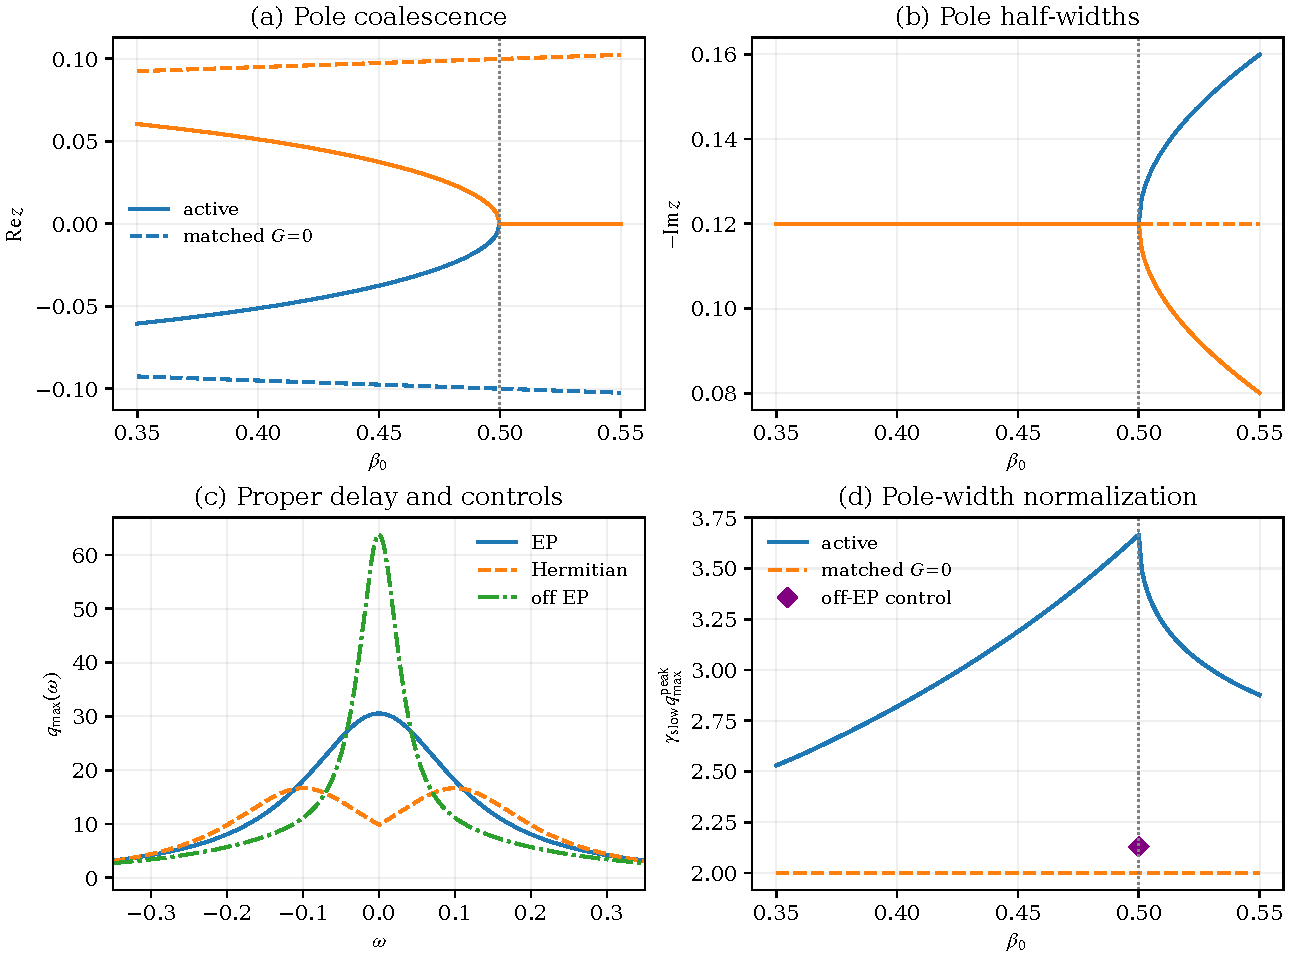
\includegraphics[width=0.92\textwidth]{SFig2_smith_delay.pdf}
\caption{%
\textbf{Causal Smith-delay validation and adverse controls.}
Panel (a) tracks the analytic pole pair to the exact core EP at
$\beta_0=0.50$.  Panel (b) shows the two pole half-widths: they remain
positive throughout the retained window and split only on the relative-broken
side.  Panel (c) compares the largest proper-delay peak with a Hermitian
control matched by total rate and with an off-EP kernel of the same total
rate ($D=0.05$); the latter exceeds the EP peak because one of its poles
decays at only $0.0334$.  Panel (d) multiplies the largest proper delay by the slowest pole
half-width $\gamma_{\rm slow}=\min_a[-\operatorname{Im}z_a]$.
The separate off-EP control is marked at $\beta_0=0.50$.
The passivity floor $\bar\Gamma-|\Gamma_{\rm PT}|$ is not used as a pole width.  Together with the unitarity and trace-delay checks,
these controls establish the proper delay as a causal coalescence and
linewidth fingerprint, not a Kondo-scale multiplier.
}
\label{fig:S_smith}
\end{figure*}

At the EP, $D=G$ and the pole pair coalesces at
$E_{\rm EP}=-i\bar\Gamma$.  The complete Jordan resolvent gives
\begin{equation}
\operatorname{Tr}Q_{\rm EP}(\omega)
=\frac{4\bar\Gamma}{\omega^2+\bar\Gamma^2},
\qquad
\int\frac{d\omega}{2\pi}\operatorname{Tr}Q_{\rm EP}=2 .
\label{eq:smith_ep_app}
\end{equation}
For $\bar\Gamma=0.12$, this predicts
$\operatorname{Tr}Q_{\rm EP}(0)=33.3333333$, reproduced numerically to
machine precision.  The finite-window numerical integral is $1.99236$; the
small deficit is the omitted Lorentzian tail.  Across the validation grid,
the maximum scattering-unitarity error is $1.33\times10^{-15}$, the maximum
Smith-Hermiticity error is $2.52\times10^{-14}$, and the maximum discrepancy
in Eq.~(\ref{eq:smith_det}) is $4.97\times10^{-14}$.

Figure~\ref{fig:S_smith} includes the essential adverse control.  An
off-EP kernel with the same total rate and $D=0.05$ reaches a largest
proper-delay peak $63.77$, exceeding the EP value $30.56$, because one of its
poles decays at only $0.0334$.  Normalized by the slowest pole half-width (both EP
poles have half-width $0.12$), the largest proper delay is $3.667$ at the EP,
$2.000$ for the Hermitian control, and $2.130$ for the off-EP kernel, so the
EP value is $1.83$ and $1.72$ times larger.  Figure~\ref{fig:S_smith}(d)
uses these pole half-widths consistently.  The trace delay, by contrast, is the same at the EP and at the
Hermitian degeneracy, $\operatorname{Tr}Q(0)=4/\bar\Gamma=33.33$, because it
depends only on the pole positions.  The proper delay therefore resolves the
coalescence; it is used as a causal coalescence and linewidth fingerprint,
not as an independent many-body amplification factor.

\section{Causal Spectral Density and a Matrix Flow Diagnostic}
\label{app:matrix_rg}

This appendix records the complete Green-function matrix analysis used for
Supplemental Fig.~\ref{fig:S_causal_rg}.  It applies the one-loop
matrix recursion patterned on poor-man's scaling~\cite{anderson1970poor}
to the positive impurity spectral matrix.  That matrix is not the bath spin
density entering a derived Kondo RG equation.  The calculation is an
operational spectral-weight diagnostic throughout this appendix.

\begin{figure*}[tbp]
\centering
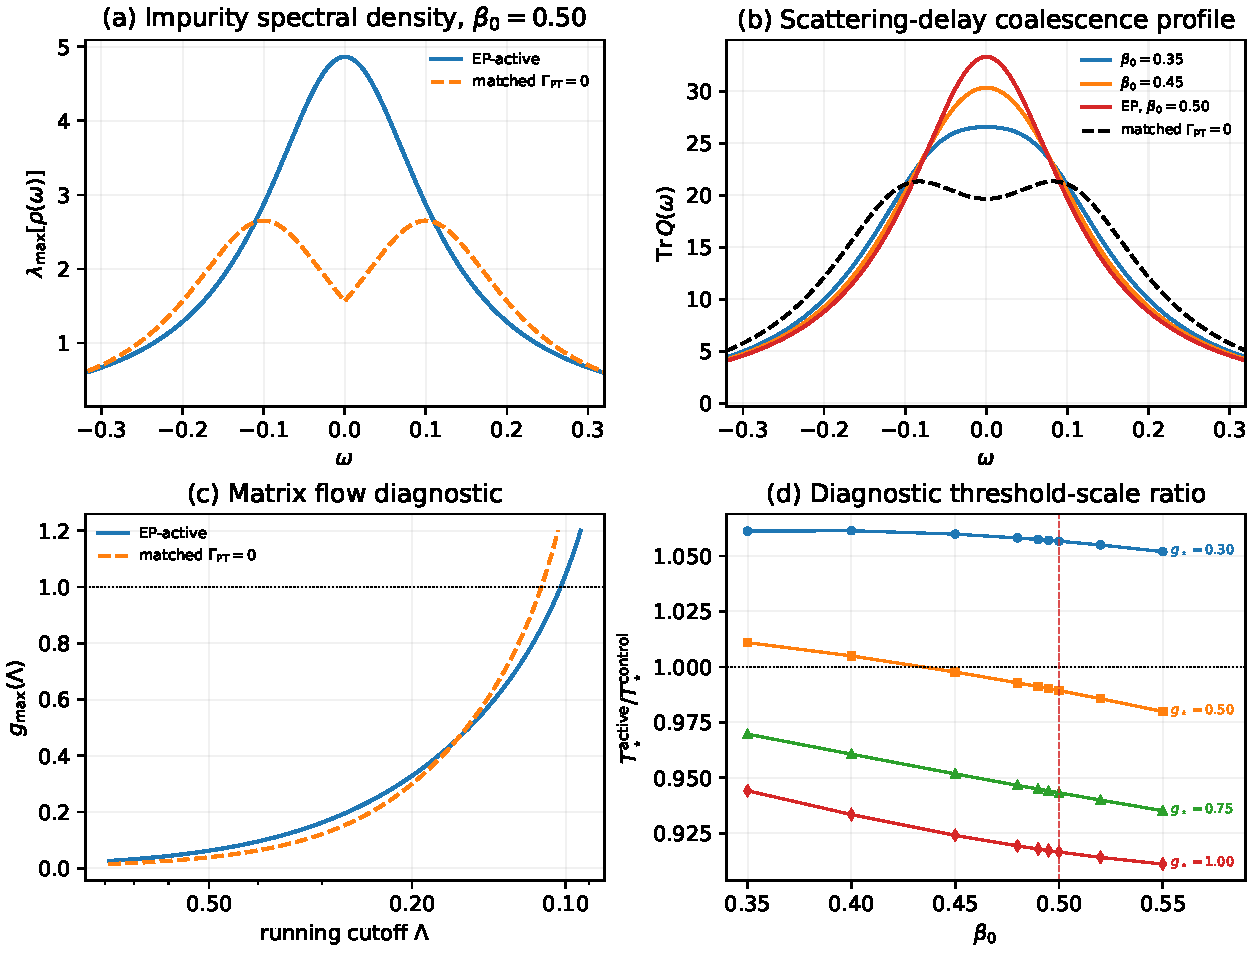
\includegraphics[width=0.92\textwidth]{SFig3_causal_rg.pdf}
\caption{%
\textbf{Causal scattering and spectral-density flow diagnostic.}
The fixed-$W$ validation uses the positive impurity spectral matrix
built from $G^R$ and $G^A$ as the channel density (App.~\ref{app:matrix_rg}),
with $\Gamma_0=0.12$ and unit charge gap.
Panel (a) compares the largest causal channel-density eigenvalue at
$\beta_0=0.50$ with the matched $\Gamma_{\rm PT}=0$ control.
Panel (b) gives the Wigner--Smith trace; the passive Fisher--Lee matrix is
unitary to $1.33\times10^{-15}$ and
$\operatorname{Tr}Q(0)=4/\Gamma_0=33.3333$ at the EP.
Panels (c) and (d) show that the EP-active exchange eigenvalue is initially
larger, but its threshold-scale ratio crosses below the control before strong
coupling.  This supports a bounded early-flow ordering of this diagnostic, not
an enhanced thermodynamic Kondo temperature.
}
\label{fig:S_causal_rg}
\end{figure*}

\subsection{Positive matrix density}

For either the spin or chiral representation,
\begin{align}
\rho_\nu(\omega)
&=\frac{i}{2\pi}\left[G_\nu^R(\omega)-G_\nu^A(\omega)\right]\nonumber\\
&=\frac{1}{2\pi}G_\nu^R(\omega)\Gamma_\nu(\omega)
G_\nu^A(\omega),\qquad \nu=s,\chi .
\label{eq:rho_matrix_rg}
\end{align}
The second equality is the retarded/advanced Dyson identity.  It proves
positivity directly: $v^\dagger\rho_\nu v =\frac{1}{2\pi} \left\|\Gamma_\nu^{1/2}G_\nu^Av\right\|^2\geq0$.
It also makes basis covariance explicit,
$\rho_\chi=U_H^\dagger\rho_sU_H$.  Consequently the two density
eigenvalues are independent of whether the calculation is displayed in
the spin or fixed chiral basis.

\subsection{Exchange matrix and flow}

We initialize the diagnostic with the conventional scalar
Schrieffer--Wolff reference value,
\begin{equation}
J_0=2W^2\left(
\frac{1}{|\epsilon_d|}
+\frac{1}{|\epsilon_d+U|}
\right)I .
\label{eq:J0_matrix_rg}
\end{equation}
Let $\ell=\ln(D_{\rm uv}/\Lambda)$ and define the symmetric shell density $\rho_{\rm sh}(\Lambda) =\rho(+\Lambda)+\rho(-\Lambda)$.
The matrix recursion integrated in this diagnostic is
\begin{equation}
\frac{dJ}{d\ell}
=J(\ell)\rho_{\rm sh}(\Lambda)J(\ell).
\label{eq:matrix_poor_man_flow}
\end{equation}
No simultaneous diagonalization of $J$ and $\rho_{\rm sh}$ is assumed.
For Hermitian $J$ and positive Hermitian $\rho_{\rm sh}$,
$J\rho_{\rm sh}J$ is Hermitian, so the flow preserves Hermiticity.
Under a fixed unitary basis change, $J\mapsto U^\dagger JU$ and
$\rho\mapsto U^\dagger\rho U$, making
Eq.~(\ref{eq:matrix_poor_man_flow}) covariant.

To compare channels without assigning significance to a basis component,
the code forms $\rho_{\rm av}=\rho_{\rm sh}/2$ and $g=\rho_{\rm av}^{1/2}J\rho_{\rm av}^{1/2}$, and follows $g_{\max}=\lambda_{\max}(g)$.
The operational scale $T_\ast(g_\ast)$ is the cutoff at which $g_{\max}(\Lambda)$ first reaches a specified threshold $g_\ast$.
It is deliberately called an operational weak-flow scale, not a
thermodynamic Kondo temperature.

\subsection{Coefficient and convergence audit}

For $k_{\rm max}=\pi/4$ the gate uses the one-dimensional normalization
$\rho_{\rm ref}=1/(2k_{\rm max})=0.637$ (the radial density of the quadratic
bath would be $1/(2\pi\alpha_{\rm b})=0.159$), $\Gamma_0=\pi\rho_{\rm ref}W^2=0.12$, and therefore, with $\epsilon_d=-1$
and $U=2$ in Eq.~(\ref{eq:J0_matrix_rg}), $W^2=0.06$ and $J_0=0.24$.
At $\beta_0=0.50$, $D_0=G_0=0.10$ and the two rate eigenvalues are
$0.04$ and $0.44$.  The selected-grid minimum density eigenvalue is
$0.0365034$, while the strict pre-EP-window minimum is
$0.0241015>0$.  The maximum difference between the two forms
of Eq.~(\ref{eq:rho_matrix_rg}) is $1.79\times10^{-15}$, the exchange
Hermiticity error is zero, and the maximum step-refinement drift is
$5.92\times10^{-10}$.

The active/control threshold-scale ratios at $\beta_0=0.50$ are
$1.0567$, $1.0179$, $0.9893$, and $0.9166$ for
$g_\ast=0.30$, $0.40$, $0.50$, and $1.00$, respectively.  The ordering
therefore reverses near $g_\ast=0.4627$.  The calculation establishes a
bounded early-flow ordering, but not a threshold-independent
enhancement of the strong-coupling Kondo scale.  In this flow $\rho_\nu$ of
Eq.~(\ref{eq:rho_matrix_rg}) is the impurity spectral matrix of the projected
kernel, used in place of the bath spin density at the impurity site that
enters a poor-man's-scaling equation.  Because $J_0\propto I$
[Eq.~(\ref{eq:J0_matrix_rg})], every EP dependence of the flow, including
these ratios, enters through that substitution.  The ratios are therefore an
operational diagnostic of the impurity resolvent; a Kondo-flow statement would
require the bath spin density.

\section{Finite-\texorpdfstring{$U$}{U} Biorthogonal NRG Residue Audit}
\label{app:nrg_jordan}

We next test the Jordan response by an operator-resolved non-Hermitian NRG
calculation in the scalar-hybridization Wilson-chain control of the projected
model~\cite{burke2025non}.  This is a weak-coupling structural control of the
local finite-$U$ residue in the early Wilson shells, not a low-energy fixed
point or a phase diagram for the full SOC-resolved bath.  It therefore
neither locates nor excludes the interacting continuation of the full-$k$
causal pole EP.  That distinct problem is addressed by the exact finite-chain
matrix block-Wilson calculation of Sec.~\ref{app:finiteU_fullk} and by the
continuum saddle of App.~\ref{app:KR}.  The present
section instead asks whether the scalar Markov-core transition residue retains
the nilpotent matrix direction.  The
two transition operators are propagated independently as
$L^\dagger cR$ and $L^\dagger c^\dagger R$; a no-truncation regression checks
their noninteracting matrix elements before the interacting scan.

\begin{figure*}[tbp]
\centering
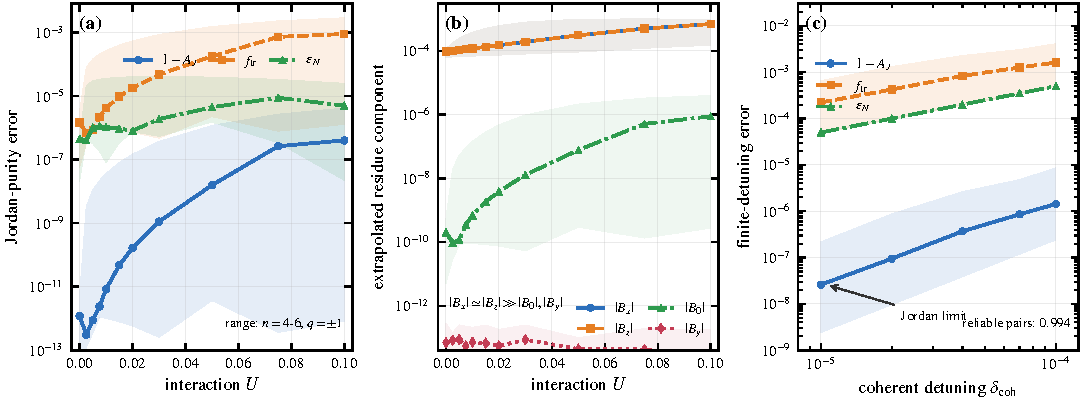
\includegraphics[width=0.98\textwidth]{SFig4_nrg_residue.pdf}
\caption{%
\textbf{Finite-$U$ Jordan transition-residue audit for the
scalar-hybridization NRG control.}
(a) Zero-detuning extrapolations of the alignment error $1-A_J$, trace
fraction $f_{\rm tr}$, and nilpotent mismatch $\epsilon_N$.  Curves are
medians and bands are the full range over the early/high-energy iterations
$n=4$--$6$ and charge
sectors $q=\pm1$.  (b) Pauli components of the extrapolated double-pole
coefficient $B$: $|B_x|\simeq|B_z|\gg|B_0|,|B_y|$, as required by
$N_{\rm EP}=\Deff\sigma_z+i\Gpt\sigma_x$.  (c) Direct finite-detuning
convergence; curves are medians and bands are the 16th--84th percentile over $U$, iteration, and tracked sector.  The reliable-pair fraction is $0.994$.
Parameters are $\Lambda=3$, $z=0.5$, $N_{\rm keep}=320$, $r=1$,
$\beta_0=0.50$, $\Deff=\Gpt=0.10$, and $0\leq U\leq0.10$.  The figure
establishes persistence of the nilpotent matrix-residue direction in this
weak-coupling structural window; it does not establish a low-energy fixed
point, pole coalescence, a universal interaction law, a thermodynamic Kondo
scale, or a phase boundary.
}
\label{fig:S_NRG_Jordan}
\end{figure*}

At the exact Jordan point a complete biorthogonal eigenbasis is singular.
We therefore calculate at finite coherent detuning
$\delta_{\rm coh}>0$, track the same two impurity-supported poles through
$U$ and $\delta_{\rm coh}$, and only then extrapolate to
$\delta_{\rm coh}\to0$.  If
\begin{equation}
G(z)=\frac{W_+}{z-z_+}+\frac{W_-}{z-z_-}+G_{\rm reg}(z),
\end{equation}
the coefficient that approaches the Jordan double-pole residue is
\begin{equation}
B=\frac{1}{2}(W_+-W_-)(z_+-z_-)
 =B_0 I+B_x\sigma_x+B_y\sigma_y+B_z\sigma_z .
\label{eq:nrg_double_pole_B}
\end{equation}
In the Hadamard/chiral basis used by the Wilson-chain adapter, the compensated
EP generator is $N_{\rm EP}=\Deff\sigma_z+i\Gpt\sigma_x$, with $N_{\rm EP}^2=0$.
We monitor the Frobenius-angle alignment, normalized trace, and nilpotent
component mismatch,
\begin{align}
A_J&=\frac{|\operatorname{Tr}(N_{\rm EP}^\dagger B)|}
{\|N_{\rm EP}\|_F\|B\|_F},\nonumber\\
f_{\rm tr}&=\frac{|\operatorname{Tr}B|}{\sqrt{2}\|B\|_F},
&
\epsilon_N&=\frac{|B_x-iB_z|}{|B_x|+|B_z|}.
\label{eq:nrg_jordan_diagnostics}
\end{align}

Supplemental Fig.~\ref{fig:S_NRG_Jordan} reports the validated part of the
audit.  The reference calculation uses $\Lambda=3$, $z=0.5$, $N_{\rm keep}=320$, bath exponent $r=1$,
$\beta_0=0.50$, $\Deff=\Gpt=0.10$, $0\leq U\leq0.10$, and the
early/high-energy NRG iterations $n=4$--$6$ in charge sectors $q=\pm1$.
Five detunings between
$10^{-5}$ and $10^{-4}$ are used.  The reliable tracked-pair fraction is
$0.993939$.  Across 328 reliable direct finite-detuning rows the median
alignment is $0.9999997628$, the median trace fraction is
$5.77076387\times10^{-4}$ and the median mismatch is
$1.99999992\times10^{-4}$.  The separate ensemble of 326 extrapolation fits
has median extrapolated mismatch $7.31791124\times10^{-7}$; its medians of
input-window alignment and trace-fraction medians are $0.9999996308$ and
$8.35670512\times10^{-4}$.  These are different statistical populations.
Both support a nearly traceless nilpotent residue direction within the
tested window.

\emph{Symmetry content.}  In this control the bath and
$Un_\uparrow n_\downarrow$ are spin-rotation invariant, and the core is a
complex impurity field $\bm B\cdot\bm\sigma$.  Complex-spin covariance
constrains the characteristic polynomial through $\bm B\cdot\bm B$; its
null-field condition remains $\Deff=\Gpt$.  Where the response is analytic,
the Green function at that condition has the form $g_0I+g_1N_{\rm EP}$.
Covariance fixes the direction of a nonzero nilpotent component, but does
not alone prove a nonzero double-pole residue of a selected resonance for
every $U$.  In particular, normalized alignment can approach one even if
the residue amplitude tends to zero.  The measured alignment therefore
checks the transition-operator calculation in the stated window; it is not
a theorem of interaction-protected pole coalescence.  Three-site exact
diagonalization at $U=8$ checks spectral covariance against a field
$(\bm B\cdot\bm B)^{1/2}\sigma_z$ to $10^{-13}$ in the three-, four- and
five-electron sectors.  The spin-asymmetric full-$k$ bath is instead treated
in Apps.~\ref{app:finiteU_fullk} and~\ref{app:KR}.

\subsection{An exact interacting comparison with a scalar bath}
\label{app:exact_PT_control}
To distinguish symmetry-fixed direction from a nonzero residue, consider
a separate finite Anderson control with spin-independent bath hopping and
hybridization, and an imposed local field
$N=\Delta\sigma_x+i\gamma\sigma_z$. It is not a replacement for the
stationary SOC bath: making that bath scalar would remove the relative-decay
mechanism, and inserting $N$ on the impurity changes the model. Related
interaction-stable symmetry-protected EPs are known~\cite{Schafer2022}.

For an isolated singlet of the Hermitian reference, define the response by
biorthogonal analytic continuation of that state. Complex-spin covariance
gives $G(z)=g_0(z)I+g_1(z)N$ at $\gamma=\Delta>0$, where $N^2=0$.
For an isolated spin-doublet transition of energy $\omega_\ell$, let
$Z_\ell$ be its per-spin spectral weight and
$m_\ell=\partial_h\omega_{\ell,\uparrow}(h)|_{h=0}$ its response to a
local real field $h(n_{d\uparrow}-n_{d\downarrow})$. Differentiating the
Hermitian spin-resolved pole gives the double-pole coefficient
$B_\ell=Z_\ell m_\ell N$. Thus nonzero $Z_\ell m_\ell$, not normalized
alignment alone, supplies the missing condition. For $K=G^{-1}$,
$K(\omega_\ell)=-(m_\ell/Z_\ell)N$ has rank one and
$\det K=(z-\omega_\ell)^2/Z_\ell^2+O((z-\omega_\ell)^3)$.

For a half-filled dimer with one bath site at zero energy, hopping $V>0$
and $\epsilon_d=-U/2$, define $a=\sqrt{U^2/16+V^2}$,
$c=\sqrt{U^2/16+4V^2}$ and $\omega_{\ell,h}=c\mp a$. Direct
diagonalization gives
\begin{equation}
 Z_\ell=\frac{\omega_\ell^2-9V^2}{2(\omega_\ell^2-\omega_h^2)},
 \qquad m_\ell=\frac12\left(1+\frac{U}{4a}\right).
 \label{eq:exact_control_residue}
\end{equation}
Both are positive for every finite $U\ge0$. The scalar Green function is
$g_0=[z-V^2/z-(U^2/4)z/(z^2-9V^2)]^{-1}$, so a dynamical interaction
self-energy is retained. Its nilpotent component is also nonzero in
general: $\Sigma_1=g_1/g_0^2-1$, rather than a frozen scalar ansatz.
The reference has $n_d=1$ and
$D_d=[1-U/\sqrt{U^2+64V^2}]/4$. The double pole persists at every finite
$U$, although $Z_\ell m_\ell\sim18V^2/U^2$ tends to zero at fixed $V$.

Fourteen untruncated checks cover one and three bath sites at
$U=0,0.5,2,4,8,16$ and five sites at $U=4,8$, with all hoppings $0.5$ and
$\Delta=\gamma=0.1$. Direct contour residues agree with $Z_\ell m_\ell$
within $2.1\times10^{-15}$; the selected charge-sector nullities of $H-E$
and $(H-E)^2$ are one and two. For five bath sites at $U=8$,
$n_d=1$, $D_d=0.01603$ and $Z_\ell m_\ell=0.02548$. Two-sided splitting
and pole-exchange loops are verified at $U=4,8$ with three bath sites.
Here internal PT means spin exchange on every site followed by complex
conjugation. A real bath $\sigma_x$ field preserves it but splits the poles
at the old null-field condition, showing that PT alone does not pin the EP.
These are finite-system, biorthogonal response statements; no passive
microscopic realization, continuum resonance or Kondo screening follows.

\paragraph{Limits of the original NRG scan.}
The stronger pole-splitting claims do not pass the same convergence gate.
Across iteration, sector, fitting window, and detuning model, the complex
interaction-exponent ensemble has median $p=1.359$ with a $68\%$ spread of
$1.991$.  The proposed complex quartic coefficient also fails its plateau
test (median absolute log-slope $0.880$ and relative complex scatter
$1.118$).  These failures do not prove the absence of a scaling regime, but
they preclude extracting a universal exponent, quartic coefficient, or
interaction-induced EP floor from this calculation.  Accordingly only the
matrix-residue result is used in the main text.

\section{Scope and Division of Labor}
\label{app:YBE}

Four statements are kept separate.  (i) For the complete frozen retarded
kernel the exact claims are the matrix Fisher--Lee relation, one-particle
contact-phase quantization, and the Wigner--Smith identity; they require no
many-body factorization.  (ii) Only after equal-velocity branchwise
linearization and folding, with constant \(M\), scalar hybridization, and
component-symmetric local \(U\), is the two-electron contact matrix
Eq.~(\ref{eq:Anderson_R_app}); its difference form and \(GL(2,\mathbb C)\)
covariance give the YBE, and, under the companion finite-ring contact and boundary assumptions,
the global nilpotent deformation retains its Jordan structure at finite $U$.  Curvature, unequal folded velocities, energy-dependent
$M(\omega)$, nonscalar hybridization, or component-dependent interactions
break (ii) and can shift or split the EP.  (iii) The finite-volume
continuation (twisted RTT relations, commuting transfer matrices, many-body
Jordan blocks, and the four-state Fock lift, whose descendant \emph{spin}
roots meet at the projective point \(\lambda=\infty\); no finite Anderson
charge-root coalescence is asserted) is taken from
Ref.~\cite{KulkarniYB2026} and is not rederived here.  (iv) The interacting
statements about the full-$k$ pole EP are numerical: the embedding from exact finite-chain
responses in App.~\ref{app:finiteU_fullk} and the mean-field saddle of
App.~\ref{app:KR}; the residue audit of App.~\ref{app:nrg_jordan} tests a
symmetric control.

\section{Finite-\texorpdfstring{$U$}{U} Kotliar--Ruckenstein saddle of the continuum bath}
\label{app:KR}

This appendix specifies the finite-$U$ saddle of main
Sec.~\ref{M-sec:finiteU_KR} and records its checks.  It is a mean-field
approximation to the interacting impurity, applied to the exact stationary
bath of App.~\ref{app:full_k_causal_ep}.  The state is the $T=0$
grand-canonical ground state of the rotating-frame Hamiltonian at chemical
potential $\mu$, the same preparation assumption as App.~\ref{app:finiteU_fullk};
the retarded $U=0$ certificate does not need it.  The parameters are those of
Eq.~(\ref{eq:app_full_k_witness_parameters}); $\bar\Gamma_0=W^2/4=0.0025$ at
$W=0.10$.

\subsection{Saddle}
Local configuration probabilities $(e,p_+,p_-,d)$ with $e+p_++p_-+d=1$ are
defined in a natural spin basis rotated by an angle $\theta$ in the real
$(x,z)$ plane, $\hat n_\theta=\sin\theta\,\sigma_x+\cos\theta\,\sigma_z$.  With $n_\pm=p_\pm+d$,
\begin{gather}
r_\pm=\frac{\sqrt{e\,p_\pm}+\sqrt{p_\mp\,d}}{\sqrt{n_\pm(1-n_\pm)}},
\label{eq:app_KR_r}\\
R=\tfrac12(r_++r_-)I+\tfrac12(r_+-r_-)\hat n_\theta,\qquad
n=\tfrac12(n_++n_-)I+\tfrac12(n_+-n_-)\hat n_\theta .
\label{eq:app_KR_R}
\end{gather}
A real symmetric field $\Lambda_f=\Lambda_{f0}I+\vec\Lambda_f\cdot\vec\sigma$, $\vec\Lambda_f=(\Lambda_{fx},0,\Lambda_{fz})$,
enforces $n_f=n$, where
\begin{equation}
n_f=\tfrac12I+\frac1\pi\int_0^\infty dy\,{\rm Herm}\,G_f(\mu+iy),\qquad
G_f(z)=\big[zI-\Lambda_f-R\,\Sigma_d^{\rm I}(z)\,R\big]^{-1},
\label{eq:app_KR_nf}
\end{equation}
and $\Sigma_d^{\rm I}$ is Eq.~(\ref{eq:app_full_k_selfenergy}) with the
static spin-even subtraction of App.~\ref{app:full_k_causal_ep}.  The saddle is
a stationary point of
\begin{equation}
\mathcal L=\Omega_{\rm qp}(R,\Lambda_f)
+\operatorname{Tr}\big[(\epsilon_dI-\Lambda_f)\,n\big]+U\,d ,
\label{eq:app_KR_L}
\end{equation}
where $\Omega_{\rm qp}$ is the $T=0$ grand potential of quasiparticles with
propagator $G_f$.  Stationarity in $\Lambda_f$ gives $n_f=n$.  Stationarity in
the three independent probabilities and in $\theta$ gives the force
equations, which contain the bath force
\begin{equation}
B=\frac{\partial\Omega_{\rm qp}}{\partial R}
=\frac1\pi\int_0^\infty dy\,{\rm Re}\big[\Sigma_d^{\rm I}RG_f
+G_fR\,\Sigma_d^{\rm I}\big]_{z=\mu+iy}.
\label{eq:app_KR_B}
\end{equation}
No paramagnetic, scalar-$Z$ or Markov restriction is imposed.  The $\theta$
equation is divided by the spin-density amplitude $(p_+-p_-)/2$; this removes
spurious unpolarized roots of the polar coordinate.  The omitted complex spin
direction is odd under complex conjugation of this real Hamiltonian and is
tested separately for stability.

\subsection{Resonance poles and EP equations}
For complex $z$ the saddle is held fixed and the bath kernel is continued to
the outgoing sheet,
\begin{equation}
K_f^{\rm II}(z)=zI-\Lambda_f-R\,\Sigma_d^{\rm II}(z)\,R,\qquad
F_{\rm KR}=\det K_f^{\rm II},\qquad
G^{\rm II}_{d,\rm coh}=R\,[K_f^{\rm II}]^{-1}R,
\label{eq:app_KR_pole}
\end{equation}
with $\Sigma_d^{\rm II}$ of Eq.~(\ref{eq:app_two_cut_sheet}) and both open
channels continued.  Since $\det K_f^{\rm II}=(\det R)^2\det[R^{-1}(zI-\Lambda_f)R^{-1}-\Sigma_d^{\rm II}]$,
the saddle acts as the linear self-energy
\begin{equation}
\Sigma_{\rm KR}(z)=(z-\epsilon_d)I-R^{-1}(zI-\Lambda_f)R^{-1}
\label{eq:app_KR_sigma}
\end{equation}
with Dyson convention $G_{d,\rm coh}^{-1}=(z-\epsilon_d)I-\Sigma_d-\Sigma_{\rm KR}$.
In particular, $R=I$ and $\Lambda_f=\epsilon_dI+\Sigma_{\rm HF}$ give
$\Sigma_{\rm KR}=\Sigma_{\rm HF}$.  The
EP equations $F_{\rm KR}=\partial_zF_{\rm KR}=0$ are solved jointly with the
saddle for $(z,\epsilon_d,V_O)$ at fixed $W$, or for $(z,\epsilon_d,W)$ at fixed
$V_O$.  At mean filling one, $\mu$ is an additional unknown with $\operatorname{Tr}n=1$.  The coherent weight of $G_{d,\rm coh}$ is $RR^\dagger$,
not the full spectral sum, so local occupations are read from the
probabilities.  Certifying loops use the local-discriminant winding and pole
tracking of App.~\ref{app:full_k_causal_ep}, with the saddle re-solved at
every loop point.

\subsection{Implementation and checks}
Imaginary-axis integrals use Gauss--Legendre quadrature on each decade
$10^{-11}\leq y\leq10^{5}$ with analytic tails, and the radial integral is
analytic.
\begin{center}
\begin{tabular}{@{}p{0.55\columnwidth}p{0.40\columnwidth}@{}}
\toprule
Check & Result\\
\midrule
Analytic radial integral against adaptive quadrature & $1.5\times10^{-16}$\\
Density and force against a 194-dimensional Hermitian star & $1.1\times10^{-12}$ and $1.5\times10^{-14}$\\
Independent $\ln\det$ functional derivatives, including displaced states & discrepancy $\leq5.1\times10^{-10}$\\
98 accepted path records, orders 32 and 64 & $\max|\Delta R_{ij}|<5.2\times10^{-13}$; control/observable changes $<1.4\times10^{-11}$\\
Held-state check at order 96 & normalized residual $<5.2\times10^{-12}$\\
Tail cutoff $10^5\to10^6$ at three points & density change $<2.3\times10^{-16}$; force change $<4.4\times10^{-18}$\\
$U=0$ limit & $Z_\pm=1$; Eq.~(\ref{eq:app_full_k_witness_solution}) recovered; $\langle n_d\rangle=0.03468$\\
First-order rates against Hartree--Fock (App.~\ref{app:KR_HF}) & agreement to 0.01--0.7\%\\
Six perturbed seeds ($\langle n_d\rangle=1$ EP) & same saddle\\
Local stability: $\mu=0$ EPs at $U=0.02$, $0.2$; $\langle n_d\rangle=1$ EP; occupied path & constrained and transverse curvatures positive\\
\bottomrule
\end{tabular}
\end{center}
The 98 records include overlapping original and extended paths, including
all 57 occupied-path points; failed continuation attempts are excluded.
Density constraints are dimensionless, and force residuals are divided by
the fixed energy scale 0.02. These finite-grid comparisons establish
numerical convergence within the stated saddle equations, not an error
bound relative to the exact interacting problem. Positive tested
curvatures establish local stability, not a unique global minimum.

Four pole-exchange loops (the low-filling points at $U=0.02$ and $0.2$,
the fixed-$V_O$ point at $U=0.0025$, and the filling-one EP) retain their
winding and exchange on refinement from 128 to 256 intervals. At quadrature
order 64, the largest pole residual is below $5.4\times10^{-21}$ and the
largest normalized saddle residual below $6.0\times10^{-12}$. Acceptance
uses these residuals and pole tracking; solver stagnation flags are retained
in the archived records. The tests are sampled numerical certificates.

At the low-filling EPs the two smallest constrained curvatures
($2.8\times10^{-9}$ and $3.8\times10^{-7}$ at $U=0.2$) lie along the
logarithmic coordinates of the small probabilities $d$ and $p_-$; the others
are near $2\times10^{-4}$.

\subsection{First-order limit}
\label{app:KR_HF}
At $d=n_+n_-$ the factors are $r_\pm=1$ with $\partial r_\pm/\partial d=0$, so
$R=I+O(U^2)$, and stationarity gives
$\Lambda_f=\epsilon_dI+U[(\operatorname{Tr}n)I-n]+O(U^2)$: the Hartree--Fock field
of main Sec.~\ref{M-sec:finiteU_KR}.  An independent first-order calculation
inserts this field, with the $U=0$ continuum density matrix $\rho=\bigl(\begin{smallmatrix}0.032677&-0.0078\\-0.0078&0.002005\end{smallmatrix}\bigr)$,
into main Eq.~(\ref{M-eq:full_k_pole_determinant}).  The saddle reproduces its
rates:
\begin{center}
\begin{tabular}{@{}llll@{}}
\toprule
Branch & Rates & KR saddle & Hartree--Fock\\
\midrule
$\mu=0$; $(\epsilon_d,V_O)$, $W$ fixed & $d\epsilon_d/dU$, $dV_O/dU$ & $0.755$, $30.41$ & $0.761$, $30.63$\\
$\mu=0$; $(\epsilon_d,W)$, $V_O$ fixed & $d\epsilon_d/dU$, $dW/dU$ & $-0.552$, $-7.631$ & $-0.551$, $-7.631$\\
$\langle n_d\rangle=1$; $(\epsilon_d,V_O,\mu)$ & $d\epsilon_d/dU$, $dV_O/dU$, $d\mu/dU$ & $-2.625$, $-105.97$, $-2.233$ & $-2.627$, $-105.99$, $-2.235$\\
\bottomrule
\end{tabular}
\end{center}
The first KR row is a finite difference over $\Delta U=10^{-4}$; the second is
a quadratic fit to $U\leq0.001$.

\subsection{Low-filling branch and strong-\texorpdfstring{$U$}{U} certificates}
At $\mu=0$ and $W=0.10$, with $(\epsilon_d,V_O)$ retuned, every point below
passes the joint residual $<10^{-9}$, $\operatorname{Im}z<0$ and the
two-open-channel test; $|\vec\Lambda_f|$ is the traceless part of $\Lambda_f$.
\begin{center}
\begin{tabular}{@{}rrlllllll@{}}
\toprule
$U$ & $U/\bar\Gamma_0$ & $\epsilon_d$ & $V_O$ & $z_{\rm EP}$ & $\langle n_d\rangle$ & $D_d$ & $1-Z_{\min}$ & $|\vec\Lambda_f|$\\
\midrule
0      & 0    & 0.015170 & 1.21342 & $0.011973-0.002807i$ & 0.03468 & $4.7\times10^{-6}$ & 0 & 0\\
0.0005 & 0.2  & 0.015538 & 1.22820 & $0.012370-0.002795i$ & 0.03324 & $4.1\times10^{-6}$ & $4.7\times10^{-6}$ & $8.1\times10^{-6}$\\
0.0025 & 1    & 0.016802 & 1.27873 & $0.013731-0.002761i$ & 0.02907 & $2.6\times10^{-6}$ & $8.2\times10^{-5}$ & $3.3\times10^{-5}$\\
0.01   & 4    & 0.020009 & 1.40336 & $0.017153-0.002702i$ & 0.02201 & $9.7\times10^{-7}$ & $5.6\times10^{-4}$ & $8.5\times10^{-5}$\\
0.02   & 8    & 0.022660 & 1.50252 & $0.019953-0.002670i$ & 0.01833 & $4.6\times10^{-7}$ & $1.2\times10^{-3}$ & $1.2\times10^{-4}$\\
0.04   & 16   & 0.025828 & 1.61762 & $0.023276-0.002644i$ & 0.01532 & $2.0\times10^{-7}$ & $2.1\times10^{-3}$ & $1.6\times10^{-4}$\\
0.08   & 32   & 0.028989 & 1.73072 & $0.026572-0.002625i$ & 0.01320 & $7.6\times10^{-8}$ & $3.5\times10^{-3}$ & $1.9\times10^{-4}$\\
0.2    & 80   & 0.031930 & 1.83887 & $0.029627-0.002610i$ & 0.01176 & $2.0\times10^{-8}$ & $5.8\times10^{-3}$ & $2.2\times10^{-4}$\\
\bottomrule
\end{tabular}
\end{center}
The certifying loop is that of main Fig.~\ref{M-fig:full_k_certificate}
(half-widths $10^{-4}$ in $\epsilon_d$ and $10^{-2}$ in $V_O$, 128 points), with
the saddle re-solved at every point:
\begin{center}
\begin{tabular}{@{}lll@{}}
\toprule
Diagnostic & $U=0.02$ & $U=0.2$\\
\midrule
Local-discriminant winding & $+1.000000000002$ & $+1.000000000015$\\
Endpoint pole permutation & $(12)$ & $(12)$\\
Pole-separation half-winding & $+0.500000000001$ & $+0.500000000008$\\
Minimum boundary modulus & $9.69\times10^{-10}$ & $4.39\times10^{-10}$\\
Maximum phase increment & $0.402$ & $0.608$\\
Minimum $|\partial_z^2F_{\rm KR}|$ & $1.770$ & $1.829$\\
Maximum $|\partial_zF_{\rm KR}|$ at the critical points & $1.1\times10^{-15}$ & $8.8\times10^{-16}$\\
Minimum pole separation & $6.61\times10^{-5}$ & $4.38\times10^{-5}$\\
Maximum pole residual & $2.6\times10^{-21}$ & $2.1\times10^{-21}$\\
Assignment/half-separation ratio & $0.241$ & $0.345$\\
Maximum saddle residual on the loop & $5.3\times10^{-13}$ & $4.6\times10^{-12}$\\
Kernel singular values at the EP & $9.3\times10^{-4}$, $9\times10^{-19}$ & $7.7\times10^{-4}$, $4\times10^{-18}$\\
Threshold gap / pole half-width & $2.78$ & $4.15$\\
Passivity margin $\Gamma_{\min}/\bar\Gamma$ & $0.815$ & $0.847$\\
$V_O/(\epsilon_O-\Omega)$ & $0.025$ & $0.031$\\
\bottomrule
\end{tabular}
\end{center}
Both tracked poles keep two open channels on both loops.  The double
occupancy at $U=0.2$ is $0.09$ of $\det n=2.23\times10^{-7}$, while
$\langle n_d\rangle=0.0118$: the interaction is strongly repulsive but acts on a
nearly empty level.  The strong-$U$ shift is kinematic.  In the natural basis
and the low-density limit, $r_\sigma^2\simeq1-n_{\bar\sigma}$, so the
hybridization energy $K_{\bar\sigma}<0$ of one spin depends on the occupation
of the other, and stationarity raises the level of spin $\sigma$ by about
$|K_{\bar\sigma}|$.  A polarized bath makes $|K_\uparrow|\neq|K_\downarrow|$, so
this shift becomes a spin field; it is the mean-field counterpart of Haldane's
level renormalization~\cite{Haldane1978}.

\subsection{Same-bath comparison}
\label{app:KR_bath}
For the controls of App.~\ref{app:finiteU_fullk}, $(\epsilon_d,W)$ at fixed
$V_O=1.21342201$, the KR saddle was solved on each of the four $z$-shifted
12-site chains, with the chain hybridization in Eqs.~(\ref{eq:app_KR_nf})
and~(\ref{eq:app_KR_B}).  The four saddles enter the same continuum two-cut
kernel through $\langle R^{-2}\rangle z-\langle R^{-1}\Lambda_f R^{-1}\rangle$,
with the saddles and EP iterated to self-consistency.  This averages
individual approximate self-energies.  In contrast, the ED estimator is
$\langle\Sigma_jG_j\rangle\langle G_j\rangle^{-1}$, obtained by averaging
the equation-of-motion responses before taking their ratio.  These
prescriptions are generally unequal.  An independent first-order check
gives $dW/dU=-4.497758$ for the response-ratio average and $-4.501190$ for
the average-density Hartree--Fock field.  Thus the comparison retains a
small estimator difference already at first order.  The ED centers are
those of App.~\ref{app:finiteU_fullk}.
\begin{center}
\begin{tabular}{@{}llllllll@{}}
\toprule
 & \multicolumn{3}{c}{$W$} & \multicolumn{3}{c}{$\epsilon_d$} & \\
\cmidrule(lr){2-4}\cmidrule(lr){5-7}
$U$ & ED & KR, chains & KR, cont. & ED & KR, chains & KR, cont. & shift ratio $\frac{\rm KR,chains}{\rm ED}$\\
\midrule
0.0010 & 0.095777 & 0.095672 & 0.092683 & 0.014840 & 0.014834 & 0.014634 & 1.025, 1.017\\
0.0015 & 0.093859 & 0.093634 & 0.089258 & 0.014687 & 0.014675 & 0.014379 & 1.037, 1.026\\
0.0020 & 0.092057 & 0.091678 & 0.085986 & 0.014543 & 0.014521 & 0.014135 & 1.048, 1.035\\
0.0025 & 0.090363 & 0.089800 & 0.082865 & 0.014406 & 0.014373 & 0.013902 & 1.058, 1.043\\
\bottomrule
\end{tabular}
\end{center}
The last column gives the ratios of the shifts of $W$ and $\epsilon_d$.  At
$U=0.0025$ the EPs are $0.011777-0.002258i$ (ED), $0.011776-0.002228i$ (KR,
chains) and $0.011684-0.001874i$ (KR, continuum).  Quadratic fits give initial
slopes $dW/dU=-4.46$ (ED) and $-4.49$ (KR, chains), against $-4.50$ for
Hartree--Fock with the $z$-averaged chain density matrix, and
$d\epsilon_d/dU=-0.347$, $-0.348$ and $-0.347$.  The approximate slope
agreement does not remove the estimator difference described above.
The continuum-to-chain ratio of the KR shifts is
$1.68$--$1.69$ in $W$ and $1.59$--$1.60$ in $\epsilon_d$, close to the ratios of
the impurity density matrices, 1.67 for the traceless part and 1.68 for the
trace; the direction of $\vec\rho$ also differs by $5^\circ$.
These ratios quantify this KR comparison, not the unknown exact continuum
error.  The certified point is the continuum KR solution in the table;
transferring a chain method correction to it would require an additional,
unvalidated assumption.  On the interacting ellipse of App.~\ref{app:finiteU_fullk}
(half-widths $10^{-4}$ in $\epsilon_d$ and $10^{-3}$ in $W$, 128 points, saddle
re-solved) the continuum KR EP gives winding $-1$, pole exchange $(12)$ and
half-winding $-1/2$, with maximum phase increment $0.144$ and assignment ratio
$0.237$.  With $V_O$ fixed, the continuum branch continues to $U=0.02$, where
$W=0.03104$, $\epsilon_d=0.01054$, $z_{\rm EP}=0.01021-0.00025i$ and
$\langle n_d\rangle=0.0039$; the next step, $U=0.03$, did not converge and is not
counted.

\subsection{Mean filling one: fold of the EP branch}
\label{app:KR_n1}
With $W=0.10$ and $\mu$, $\epsilon_d$ and $V_O$ retuned for
$\operatorname{Tr}n=1$, the EP at $U=0.0025$ lies at
$z_{\rm EP}=0.006535-0.002983i$, with $\epsilon_d=0.008762$, $V_O=0.94586$ and
$\mu=0.006657$; the bath filling therefore differs from that of the witness.
Here $D_d=0.229$ against $\det n=0.241$, $P_1=\langle n_d\rangle-2D_d=0.542$ and
$Z_\pm=0.9974$: a charge-fluctuating state, not a local moment.  The kernel
singular values are $1.54\times10^{-3}$ and $2\times10^{-18}$.  On the loop $\epsilon_d=\epsilon_{d,\rm EP}+5\times10^{-6}\cos\phi$,
$V_O=V_{O,\rm EP}+10^{-3}\sin\phi$ with $\mu$ fixed and the saddle re-solved at
128 points, the poles exchange (error $8.5\times10^{-16}$) with half-winding
$-1/2$ [main Fig.~\ref{M-fig:KR_n1}(a)].  The smallest constrained and transverse
curvatures are $7.8\times10^{-5}$ and $8.7\times10^{-5}$.

Treating $U$ as an unknown and stepping $V_O$ gives a local maximum
$U_c=0.0030826663=1.23\bar\Gamma_0$ at $V_O=0.8566403$ and $\mu=0.0044725258$, followed by a return to smaller $U$
[main Fig.~\ref{M-fig:KR_n1}(b)].  Refinement at quadrature order 48 gives
$dU/dV_O\simeq0$, $d^2U/dV_O^2\simeq-0.615$ and a nonsingular
parameterized constraint Jacobian.  This establishes a local fold of the
exact-filling-one branch.  With $V_O$ fixed and $(\epsilon_d,W,\mu)$ retuned,
the stored continuation has a fold at $U_c=0.007948$, $W=0.1847$
[main Fig.~\ref{M-fig:KR_n1}(c)].  Both occur before a local moment develops.

The exact-filling constraint matters.  Hold $\mu=0.00447252582008$ at the
first fold, keep $W=0.10$, and solve the EP and saddle equations without
imposing $\operatorname{Tr}n=1$.  At $U=0.0032>U_c$ a fresh order-64 solve gives
\begin{gather}
\epsilon_d=0.006520501659,\qquad V_O=0.845166571137,\nonumber\\
z_{\rm EP}=0.004515007629-0.003075182314i,\qquad
\langle n_d\rangle=0.98586922,\quad D_d=0.21329561.
\label{eq:app_KR_near_one}
\end{gather}
Here $|F|=1.75\times10^{-21}$, $|F_z|=6.54\times10^{-16}$,
$F_{zz}=1.76239-0.37145i$, and the kernel singular values are
$1.72\times10^{-3}$ and $1.11\times10^{-18}$.  The smallest constrained and
transverse curvatures are positive, $9.56\times10^{-5}$ and $1.20\times10^{-4}$.  On a 128-point ellipse of radii $2\times10^{-6}$
in $\epsilon_d$ and $2\times10^{-4}$ in $V_O$, with the saddle re-solved,
the discriminant winding is $-1$, the poles exchange, and the separation
half-winding is $-1/2$.  Both channels stay open.  The maximum saddle and
pole residuals are $1.63\times10^{-15}$ and $4.98\times10^{-21}$.
Thus the constrained fold does not exclude nearby EPs at higher $U$.
The single-occupancy probability is only $P_1=0.55928$, so this is still a
charge-fluctuating state, not a local-moment EP.

The separate occupied path in Fig.~\ref{fig:S_KR_occupied} fixes $\mu=0.012$, $V_O=1.21342201$, $W=0.10$ and
$\epsilon_d=0.0151703-U/2$; it is not particle--hole symmetric in this
asymmetric bath.
\begin{center}
\setlength{\tabcolsep}{7pt}
\begin{tabular}{@{}llllll@{}}
\toprule
$U$ & $\langle n_d\rangle$ & $D_d$ & density eigenvalues & lower pole & upper resonance\\
\midrule
0.02 & 0.97580 & 0.0598 & 0.0734, 0.9024 & $0.003699-0.000306i$ & $0.019904-0.002500i$\\
0.08 & 0.98677 & 0.0067 & 0.0072, 0.9796 & $-0.025655$ (bound) & $0.049580-0.002411i$\\
0.20 & 0.99406 & 0.0013 & 0.0013, 0.9927 & $-0.085278$ (bound) & $0.108818-0.002407i$\\
\bottomrule
\end{tabular}
\end{center}
All three saddles are local minima, and the pole pairs have nonzero
$\partial_zF_{\rm KR}$.  The controls on this path do not enforce the EP
equations, so the separated poles neither establish nor exclude an
occupied-regime EP.  The large-energy poles at strong $U$ are coherent-saddle
poles, not a controlled description of Hubbard satellites.

\begin{figure*}[tbp]
\centering
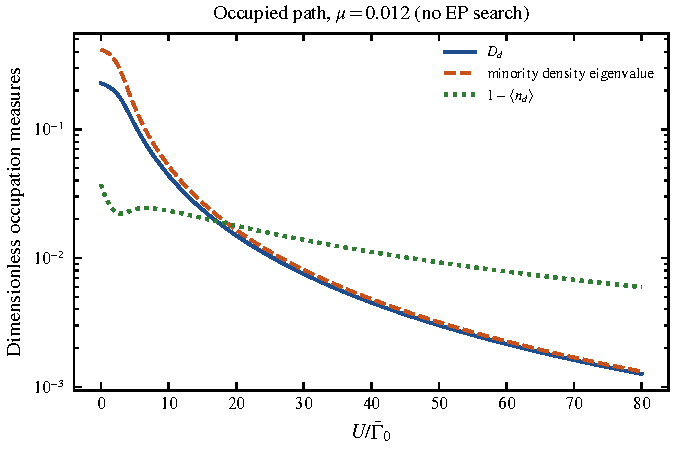
\includegraphics[width=0.64\textwidth]{SFig5_kr_occupied_path.pdf}
\caption{\textbf{Separate occupied path in the continuum KR saddle}
($T=0$).  The controls are $\mu=0.012$, $V_O=1.21342201$, $W=0.10$ and
$\epsilon_d=0.0151703-U/2$, with fixed reference width
$\bar\Gamma_0=0.0025$.  Double occupancy $D_d$, the minority eigenvalue of
the impurity density matrix, and $1-\langle n_d\rangle$ decrease along this
path.  The bath is asymmetric, so the gate prescription does not impose
particle--hole symmetry.  The EP equations are not imposed: the split poles
tabulated in App.~\ref{app:KR_n1} neither establish nor exclude an occupied
EP after retuning.  The certified filling-one EP is shown in main
Fig.~\ref{M-fig:KR_n1}.}
\label{fig:S_KR_occupied}
\end{figure*}

\subsection{Scope}
These are locally stable mean-field saddles.  They do not bound the error of
the KR approximation relative to the exact interacting impurity, prove a
global free-energy minimum, or describe a screened Kondo state: in a polarized
bath the saddle gives a field-polarized static moment rather than a Kondo
resonance with an exact width.  The tabulated chain shifts differ by at
most 6\%, including a mesh-estimator difference; this is not an error bound
for an exact continuum result.  The low-filling strong-$U$ branch remains
nearly empty.  The exactly filling-one folds concern two constrained
control families and do not exclude the nearby EP of
Eq.~(\ref{eq:app_KR_near_one}).  Testing a local-moment EP requires a
controlled interacting continuum calculation, such as matrix-bath NRG
with occupied-band convergence.

% ============================================================

\FloatBarrier
\section*{Reproducibility}
The accompanying archive contains the numerical scripts, parameter tables,
and exported data used for the main and Supplemental figures.  The public
baseline is available in the
\href{https://github.com/VMKPHYSMATH/emergent-pt-dirac-impurity}{version-controlled GitHub repository}~\cite{kulkarni2026code}.
The original numerical baseline is Release v2.1.0, archived at
\href{https://doi.org/10.5281/zenodo.21888925}{doi:10.5281/zenodo.21888925};
the all-versions record is
\href{https://doi.org/10.5281/zenodo.21434682}{doi:10.5281/zenodo.21434682}.
Release v2.1.0 includes the full-momentum certificate, SOC continuation,
finite-$U$ block-Wilson outputs, and finite-chain convergence gates reported
here.  Corrected real-frequency and Smith-delay figures and the direct
filling checks are supplied in the accompanying revision archive;
they are not contained in that earlier public snapshot. The dated 28 October revision in the
repository supplies these additions; a matching fixed-version deposit
will be identified after archiving. Its \nolinkurl{checks_20261028/}
directory contains the occupied-bath, two-sided pole, optimized-bath and
exact PT-control scripts and outputs. The PT control is explicitly a
different model and is not used to certify the driven-bath interaction
claim.
The accompanying source also includes
\nolinkurl{verify_finiteU_contact_algebra.py}, which reproduces the
finite-\(U\) \(R\)-matrix, metric covariance, and YBE residuals quoted above.
The script \nolinkurl{full_k_two_cut_ep_certificate.py} reproduces the exact
rotating-drive auxiliary closure, analytic full-momentum self-energy,
two-cut continuation, nonlinear double-zero solve, local winding, and pole
exchange of Fig.~\ref{M-fig:full_k_certificate}.
The companion script \nolinkurl{full_k_ep_soc_family.py} continues the
double-zero locus in SOC, repeats the full topological certificate at three
representative points, and generates main Fig.~\ref{M-fig:full_k_soc_family}
and its tabulated data.
The script \nolinkurl{pt_phase_diagram.py} retains its historical filename
but now evaluates the retarded upper rim and records positive half-width
checks.  With \nolinkurl{make_pt_phase_figure.py} it reproduces the
real-frequency splitting diagnostic in main Fig.~\ref{M-fig:pt_phase},
not a $\PT$ phase diagram.  The certificate module is bundled beside it.
The revision also supplies \nolinkurl{make_smith_revision.py}, the matched
filling outputs and a validation report distinguishing fresh reruns from
archived evidence.
The archived \nolinkurl{finiteU_fullk_*} JSON summaries record the exact
finite-chain interaction path, local winding, pole exchange,
equation-of-motion identity, \(N_z=4\to8\) center check, and kept-space
calibration of Sec.~\ref{app:finiteU_fullk}.
The archived \nolinkurl{fullk_n_scaling_gate_summary.json} and
\nolinkurl{FULLK_N_SCALING_AUDIT.md} record the independently optimized
$N=10$ and $12$ common-contour gate and Eq.~(\ref{eq:app_finiteU_rouche}).
The accompanying \nolinkurl{archive_additions/redraw_main_figures.py} renders
the four main figures from the retained numerical records, including the
finite-$U$ summaries.  It changes display coordinates and layout only; the pole
values and topological checks are unchanged.  The original
\nolinkurl{make_finiteU_fullk_exact_figure.py} is retained with its source
data.
The NRG archive additionally contains the independent transition-operator
propagation, no-truncation regression, branch-tracking and convergence
scripts, the gate summary, and the exported data used in
Fig.~\ref{fig:S_NRG_Jordan}.
The revision archive also contains the finite-$U$ Kotliar--Ruckenstein package
with its JSON results (\nolinkurl{matrix_saddle.py},
\nolinkurl{filling_continuation.py} and \nolinkurl{validate.py}); the
strong-$U$ certificates (\nolinkurl{kr_certificate.py}); the same-chain
comparison (\nolinkurl{kr_on_chain.py} and \nolinkurl{compare_bath.py}); the
filling-one continuation and fold (\nolinkurl{extend_n1.py} and
\nolinkurl{fold_n1.py}); the corrected $U\to\infty$ saddle with the closed form
of Eq.~(\ref{eq:app_sb_closed_form}); and \nolinkurl{make_fig5.py} and
\nolinkurl{make_filling_figures.py}, which render main
Figs.~\ref{M-fig:finiteU_KR} and~\ref{M-fig:KR_n1}, and
Fig.~\ref{fig:S_KR_occupied}, from the stored results.

% Flush bibliography control records before the legacy REVTeX end hook.
\makeatletter
\write@bibliographystyle
\makeatother
\bibliography{ref}

% Restore natbib's end-of-document consistency check under the bundled REVTeX.
\makeatletter
\NAT@swatrue\let\bibcite\NAT@testdef
\makeatother
\end{document}
